\documentclass[manuscript,screen,review]{acmart}

\usepackage{graphicx}
\usepackage{hyperref}
\usepackage[utf8]{inputenc}
\usepackage{booktabs}
\usepackage{url}
\usepackage{comment}
\usepackage{microtype}
\usepackage{siunitx}
\usepackage{subcaption}
\sisetup{output-exponent-marker=\ensuremath{\mathrm{e}}}
\usepackage{wrapfig}
\usepackage{tabularx}
\usepackage{ragged2e}


\pdfstringdefDisableCommands{%
  \def\unskip#1{<#1>}%
}

%%
%% \BibTeX command to typeset BibTeX logo in the docs
\AtBeginDocument{%
  \providecommand\BibTeX{{%
    Bib\TeX}}}

%% Rights management information.  This information is sent to you
%% when you complete the rights form.  These commands have SAMPLE
%% values in them; it is your responsibility as an author to replace
%% the commands and values with those provided to you when you
%% complete the rights form.
% \setcopyright{acmcopyright}
% \copyrightyear{2018}
% \acmYear{2018}
% \acmDOI{XXXXXXX.XXXXXXX}

%% These commands are for a PROCEEDINGS abstract or paper.
% \acmConference[Conference acronym 'XX]{Make sure to enter the correct
%   conference title from your rights confirmation email}{June 03--05,
%   2018}{Woodstock, NY}
%%
%%  Uncomment \acmBooktitle if the title of the proceedings is different
%%  from ``Proceedings of ...''!
%%
%%\acmBooktitle{Woodstock '18: ACM Symposium on Neural Gaze Detection,
%%  June 03--05, 2018, Woodstock, NY}
% \acmPrice{15.00}
% \acmISBN{978-1-4503-XXXX-X/18/06}


%%
%% Submission ID.
%% Use this when submitting an article to a sponsored event. You'll
%% receive a unique submission ID from the organizers
%% of the event, and this ID should be used as the parameter to this command.
%%\acmSubmissionID{123-A56-BU3}

\renewcommand\UrlFont{\color{blue}\rmfamily}

%%
%% end of the preamble, start of the body of the document source.
\begin{document}

% Per ACM Computing Surveys Call:

% https://dl.acm.org/journal/csur/author-guidelines

% The ACM Computing Surveys publishes surveys of and tutorials on areas of computing research or practice.
% Long paper (ours)
%   Summarizes and organizes recent research results in a novel way 
%   Integrates and adds understanding to work in the field
%   Assumes a general knowledge of the area
%   Emphasizes 
%     Classification of the existing literature
%     Developing a perspective on the area
%     Evaluating trends
% Length
%   Should normally not exceed 35 pages, including references
%   When justified, additional material may be considered or published in an electronic supplement 
%   You will need to go through the manuscript and indicate which pages will form your 35 pages for publication and which pages are for the electronic supplement
%   Manuscripts of excessive length may be rejected without review
% Use of the ACM Journals/Transactions LaTeX style is encouraged to ensure proper formatting
% A footnote on the first page should acknowledge funding sources and presentations
% Author's current address should be given in a footnote on the first page.
% 


%%
%% The "title" command has an optional parameter,
%% allowing the author to define a "short title" to be used in page headers.
\title{Examining Multimodal Methods for Analyzing Learning and Training Environments: A Systematic Literature Review}

%%
%% The "author" command and its associated commands are used to define
%% the authors and their affiliations.
%% Of note is the shared affiliation of the first two authors, and the
%% "authornote" and "authornotemark" commands
%% used to denote shared contribution to the research.

\author{Anonymous Author 1}
\email{anonymous@anonymous.edu}
\orcid{XXXX-XXXX-XXXX}
\affiliation{%
  \institution{Anonymous University}
  \streetaddress{Address}
  \city{City}
  \state{State}
  \country{Country}
  \postcode{Postal Code}
}

\author{Anonymous Author 2}
\email{anonymous@anonymous.edu}
\orcid{XXXX-XXXX-XXXX}
\affiliation{%
  \institution{Anonymous University}
  \streetaddress{Address}
  \city{City}
  \state{State}
  \country{Country}
  \postcode{Postal Code}
}

\author{Anonymous Author 3}
\email{anonymous@anonymous.edu}
\orcid{XXXX-XXXX-XXXX}
\affiliation{%
  \institution{Anonymous University}
  \streetaddress{Address}
  \city{City}
  \state{State}
  \country{Country}
  \postcode{Postal Code}
}

\author{Anonymous Author 4}
\email{anonymous@anonymous.edu}
\orcid{XXXX-XXXX-XXXX}
\affiliation{%
  \institution{Anonymous University}
  \streetaddress{Address}
  \city{City}
  \state{State}
  \country{Country}
  \postcode{Postal Code}
}

\author{Anonymous Author 5}
\email{anonymous@anonymous.edu}
\orcid{XXXX-XXXX-XXXX}
\affiliation{%
  \institution{Anonymous University}
  \streetaddress{Address}
  \city{City}
  \state{State}
  \country{Country}
  \postcode{Postal Code}
}

\author{Anonymous Author 6}
\email{anonymous@anonymous.edu}
\orcid{XXXX-XXXX-XXXX}
\affiliation{%
  \institution{Anonymous University}
  \streetaddress{Address}
  \city{City}
  \state{State}
  \country{Country}
  \postcode{Postal Code}
}

\author{Anonymous Author 7}
\email{anonymous@anonymous.edu}
\orcid{XXXX-XXXX-XXXX}
\affiliation{%
  \institution{Anonymous University}
  \streetaddress{Address}
  \city{City}
  \state{State}
  \country{Country}
  \postcode{Postal Code}
}

\renewcommand{\shortauthors}{Anonymous et al.}

% Per ACM: 
%   Abstract should be at most 100 words long and consist of short, direct sentences.
%   Should state the objectives of the work
%   Summarize the results
%   Give the principal conclusions
%   Do not use the first person
%   Do not display mathematics
%   Do not use citation reference numbers
%   Try to avoid starting with the words "This paper ..."


\begin{abstract}
As learning and training technologies continue to improve, so do our abilities to collect data from these environments and develop methods to better inform participants' learning and training processes. This allows for capturing, combining, and analyzing datastreams across several different modalities (e.g., speech, video, eye gaze, etc.) and leveraging large amounts of rich, multimodal data to help explain how individuals learn and train. In recent years, the field of multimodal learning analytics (MMLA) has grown considerably, as researchers are discovering that combining multiple modalities 1) often harnesses more predictive power, and 2) is more informative with respect to the learning and training processes, than analyzing any single modality alone. While there have been several surveys and literature reviews focusing on multimodal learning and training, they are often specific to individual pieces of the multimodal pipeline (e.g., presenting a conceptual model \cite{di_mitri_signals_2018} and data fusion \cite{chango_improving_2021}). To the best of our knowledge, no literature review has yet been conducted on the \textit{methods} used to inform multimodal learning and training environments.

In this literature review, we conduct a comprehensive analysis of the research methods currently being applied to multimodal learning and training environments. We present a taxonomy and framework that represent recent advancements in multimodal learning and training methodology, where we categorize multimodal data into five distinct subdomains: Natural Language, Vision, Sensors, Human-Centered, and Logs. We present descriptive statistics and perform an in depth qualitative, thematic analysis, and discuss our findings with respect to the current state-of-the-art, results, challenges, and research gaps for both the individual subdomains and the field as a whole. In doing so, we identify the need for an additional data fusion classification --- \textit{mid fusion} --- and introduce a novel, graph-based approach to literature review corpus distillation, which we refer to as \textit{citation graph pruning}.

\end{abstract}

%%
%% The code below is generated by the tool at http://dl.acm.org/ccs.cfm.
%% Please copy and paste the code instead of the example below.
%%

% Per ACM:

% Content Indicators

% Three types of content indicators must be assigned: (1) general terms, (2) subject descriptors, and (3) keywords and phrases. The first two items are selected from the 2012 ACM Computing Classification Scheme. Select as many of these as may be applicable.

% The keywords and phrases are additional English language words that indicate the content of the submission. They should not be synonymous with those already in the classification system: they can be more specific than the subject descriptors, or they may not be covered by the existing system at all. The following guidelines may be helpful.

%     Use important terms from the title; include their synonyms, related words and words of higher or lower generic rank.
%     Use English nouns, or noun-noun and noun-adjective combinations; do not use hyphens unless the hyphenated parts are always treated as a single unit.
%     Use specific terms whose meanings are generally accepted; do not use broad catchall terms (such as "computer", "automatic", "machine", "system", "discussion", "description"); do not use private terms or acronyms that may not be generally known.
%     Do not use negative terms stressing what your paper does not do.

% \begin{CCSXML}
% <ccs2012>
%  <concept>
%   <concept_id>10010520.10010553.10010562</concept_id>
%   <concept_desc>Computer systems organization~Embedded systems</concept_desc>
%   <concept_significance>500</concept_significance>
%  </concept>
%  <concept>
%   <concept_id>10010520.10010575.10010755</concept_id>
%   <concept_desc>Computer systems organization~Redundancy</concept_desc>
%   <concept_significance>300</concept_significance>
%  </concept>
%  <concept>
%   <concept_id>10010520.10010553.10010554</concept_id>
%   <concept_desc>Computer systems organization~Robotics</concept_desc>
%   <concept_significance>100</concept_significance>
%  </concept>
%  <concept>
%   <concept_id>10003033.10003083.10003095</concept_id>
%   <concept_desc>Networks~Network reliability</concept_desc>
%   <concept_significance>100</concept_significance>
%  </concept>
% </ccs2012>
% \end{CCSXML}

% \ccsdesc[500]{Computer systems organization~Embedded systems}
% \ccsdesc[300]{Computer systems organization~Redundancy}
% \ccsdesc{Computer systems organization~Robotics}
% \ccsdesc[100]{Networks~Network reliability}

% %
% % Keywords. The author(s) should pick words that accurately describe
% % the work being presented. Separate the keywords with commas.
\keywords{multimodal data, learning environments, training environments}

\received{00 Month 2023}
% \received[revised]{12 March 2009}
% \received[accepted]{5 June 2009}

%%
%% This command processes the author and affiliation and title
%% information and builds the first part of the formatted document.
\maketitle

% Combined introduction with background due to space constraints and repeated text

\section{Introduction and Background} \label{sec:intro_background}

% Discuss recent, past, and prominent works
\subsection{A Brief History}

Modern research in education and the learning sciences has seen a large push toward personalizing curriculum and the educational process to individual learner needs. Throughout this transformation, many methods of learner personalization and adaptation have been developed; however, among these, data-driven methods have emerged as an extremely promising approach. This research on data-driven learner personalization has come to be known as the field of learning analytics\footnote{\href{https://www.solaresearch.org/about/what-is-learning-analytics/}{https://www.solaresearch.org/about/what-is-learning-analytics/}}. Learning analytics research focuses on the collection and analysis of learner data in order to generate insights about learner behaviors \cite{maseleno2018demystifying, Zilvinskis2017}. These insights can then drive a variety of classroom tools and interventions such as computer-based learning and intelligent tutoring environments (e.g., \cite{heffernan2014assistments, leelawong2008designing}), adaptive scaffolding (e.g., \cite{Emerson2020, basu2017learner}), teacher-feedback tools (e.g., \cite{rodriguez2018teacher, Hutchins2023}), and many other developments. 

However, persistent throughout research in the field of learning analytics is the question: \textit{What forms of data need to be collected to gain insights into learner behaviors and enable meaningful analysis of learning scenarios} \cite{vatral2022using, ochoa2017multimodal}? In early learning analytics research, this question was largely answered through considerations of practicality; that is, the data which was analyzed was the data which was practical to collect in the classroom. This meant that early research on learning analytics focused highly on analyzing data from computer-based learning environments, where researchers had significant control over the design of the environments and curriculum, and log data could be easily collected and interpreted. This work analyzing log data from computer-based learning environments has a long, rich history and helped to develop meany of the theories and methods still used in learning analytics today. Log data from computer-based environments paints a very reasonable picture of learners actions and interactions in the context of the tasks they are performing in the environment that can be used to generate a wide variety of new insights into learners \cite{hoppe2017computational, ochoa2017multimodal}. 

However, as the field of learning analytics continues to advance, the limitations of these more traditional log-based analysis approaches has been the topic of significant and increased scrutiny \cite{ochoa2017multimodal}. For example, what if the learning or training environment does not facilitate easy action logging? This is certainly the case for environments which are more physical and less virtual than traditional computer-based learning and intelligent tutoring environments, such as traditional classrooms (see Section \ref{subsec:environment_type}). Beyond this, what if the logged data fails to capture the full context of learners' actions and behaviors? For example, computer logs may not tell any information about learner affect or collaborative conversations between learners. These questions, among many others, alongside the development and proliferation of affordable sensor devices, have lead learning analytics researchers to deploy additional sensor and other data collection devices in the classroom to help close the gaps introduced by the analysis of log data alone. These more complex sensors and data sources have the ability to capture a much richer variety of learner behavioral data. For example, physical movement, gestures, and postures captured through video data; dialogue captured through microphones; stress levels captured through biometric sensors; eye gaze and attention captured through eye tracking devices; etc \cite{vatral2022using}. 

By combining all of these additional sensor devices, researchers can capture a much richer picture of learners' affective, cognitive, psychomotor, and metacognitive states, leading to a more comprehensive analysis of learners' behaviors \cite{blikstein2016multimodal}. This combination of multiple sensor modalities for analysis of learner behavior has come to be known as the field of multimodal learning analytics (MMLA) \cite{blikstein2013multimodal, blikstein2016multimodal, worsley_multimodal_2018}. Today, MMLA has been the subject of over a decade of concentrated research including multiple journal special issues \cite{BJETSpecialIssue}\footnote{\href{https://www.mdpi.com/journal/sensors/special_issues/multimodal_learning_analytics_sensor}{https://www.mdpi.com/journal/sensors/special\_issues/multimodal\_learning\_analytics\_sensor}}\footnote{\href{https://learning-analytics.info/index.php/JLA/announcement/view/102}{https://learning-analytics.info/index.php/JLA/announcement/view/102}}, a special interest group in the Society for Learning Analytics Research\footnote{\href{https://www.solaresearch.org/community/sigs/crossmmla-sig/}{https://www.solaresearch.org/community/sigs/crossmmla-sig/}}, an edited book \cite{MMLAHandbook}, and several systematic literature reviews \cite{Chango2022, Alwahaby2022, Shankar2018, Crescenzi2020, Mu2020, DiMitri2018, worsley_multimodal_2018}. Owing to this significant body of prior work, in this review, we narrow our focus to the study of only applied research methods studies.

\subsection{Contributions} \label{subsec:contributions}

In this work, we perform a systematic literature review of the methods applied to multimodal learning and training environments. The scope of this review extends to any publication that both collects and analyzes data across multiple modalities or data collection mediums. This includes environments that exist fully in reality (e.g., physical therapy), mixed-reality environments (e.g., manikin-based nursing training), and online learning environments (e.g., students learning physics via computer software). Importantly, this review does not include ``virtual reality" (VR) environments due to difficulties scaling this technology in classroom settings \cite{cook2019challenges} and video data lacking semantic meaning with respect to its environment.

The novel contributions of this work are the following: 
\begin{itemize}
    \item A \textbf{comprehensive review} of the research methods applied to multimodal learning and training environments with respect to the current state-of-the-art, results, challenges, and research gaps for both modality subdomains and the field as a whole
    \item A \textbf{congruent framework and taxonomy} that reflects recent advancements in MMLA methodology
    \item An \textbf{additional data fusion classification} called \textit{mid fusion}
    \item A \textbf{corpus reduction procedure} via a citation graph and graph-based algorithms, which we refer to as \textit{citation graph pruning}
\end{itemize}

\subsection{Related Work} \label{subsec:related_work}
% EDUARDO 

% Other literature reviews
% How are we different than others?
% Other lit reviews/surveys:
%   A review on data fusion in multimodal learning analytics and educational data mining
%   Multimodal data capabilities for learning: What can multimodal data tell us about learning?
%   Trends of Multimodal Learning Analytics: A Systematic Literature Review
Following this recent wave of MMLA research, surveys and literature reviews have portrayed the MMLA landscape through various windows. Concisely, some of these include: multimodal data fusion \cite{chango_review_nodate}, conceptual model and taxonomy \cite{di_mitri_signals_2018}, statistical and qualitative assessment of literature \cite{sharma_multimodal_2020, qushem_trends_nodate}, virtual reality \cite{philippe_multimodal_2020}, technology and data engineering focused for automating MMLA \cite{chua_technologies_2019}, and impact and ethical considerations \cite{alwahaby_evidence_2021}. Our literature review augments these by focusing on the applied methods currently being used to inform multimodal learning and training environments. While prior works have touched on this, no recent works (to our knowledge) have explicitly centered on multimodal learning and training methodology. In the following paragraphs, we detail two foundational reviews from which we derived our own review's framing. Our intention is to extend and modify these existing taxonomies to reflect recent MMLA advancements. 

% DI MITRI (Observability)
%   From signals to knowledge: A conceptual model for multimodal learning analytics
In a \citet{di_mitri_signals_2018} review, the authors proposed the Multimodal Learning Analytics Model (MLeAM), a conceptual model that describes the cyclical relationship between behavior, data, machine learning, and feedback in MMLA. Along with a comprehensive taxonomy, a key contribution was the idea of data observability and its splitting of space into input and hypothesis. Specifically, \citet{di_mitri_signals_2018} states that there is an observability line acting as the boundary between these two spaces, where input space is for measurable and sensory evidence (e.g., behaviors) and the hypothesis space is reserved for human-inferred annotation (e.g., emotions, motivation, cognition, and belief). This idea of observability, which refers to the process of using AI to turn input evidence into hypotheses, has guided our understanding as we define and describe applied MMLA research through this lens.

% CHANGO: (Data Fusion)
%   A review on data fusion in multimodal learning analytics and educational data mining
%   Fusion of multiple modalities and its affects in ML and EDM
%   Focus on the data fusion itself
%   Modalities mentioned: audio, video, electrodermal activity, gaze, logs, clicks, gestures, speech, writing
%   Hardware mentioned: computers, cameras, sensors, infrared imaging, eye tracking glasses
%   Used SLR template from Tranfield 2003, not Kitchenham
%   Does not have the granularity we are discussing, so currently no conflicts with our definitions
%   5 categories of data: digital, e.g. clicks and logs; physical, e.g. gestures; physiological, e.g. EEG; psychometric, e.g. mental state surveys; environmental, e.g. physical location, temperature, weather
%   Capture methods: webcam, eye trackers, electrodes, sensors, .csv files, software
%   Data collected across: data source, data type, data category, capture method
%   Fusion: early fusion (feature level, before analysis), late fusion (decision level, after analysis), hybrid
Another influential survey is by \citet{chango_review_nodate}, which focuses on fusion methodologies and practices in MMLA. In the review, the authors classify papers by data fusion technique and point, aiming to understand fusion's impact on machine learning methods in educational data mining. After generating and reading their corpus, they proposed a classification scheme defining three types of data fusion --- \textit{early}, \textit{late}, or \textit{hybrid} --- depending on the stage of integration. Early fusion involves \textit{feature-level} concatenation prior to classification, while late fusion refers to \textit{decision-level} concatenation after classification. Hybrid fusion employs a mixture of both early and late fusion.

Combining the taxonomies from both reviews, an adapted classification scheme emerges for data fusion that centers upon the idea of \textit{feature observability}, which can be used to identify the different processes by which individuals fuse different sources of information to create unified data representations. This definition also accounts for the distinction between measurable sensory evidence and human-inferred annotations, guided by the observability line. In the upcoming section, we elaborate on this data fusion classification scheme and present our refined taxonomy.

\section{Framework and Taxonomy}

\subsection{Framework} \label{sec:framework}

% Lens through which we are conducting this research
% Framework diagram and explanation
\begin{figure}[htbp]
    \centering
    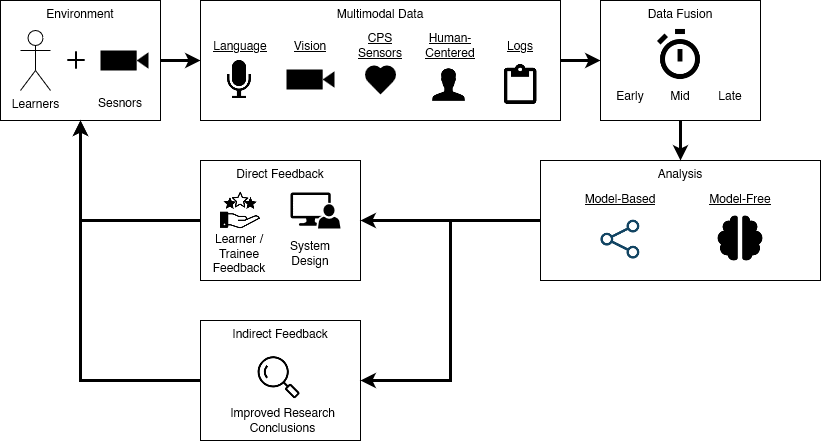
\includegraphics[width=0.9\textwidth]{img/MMLTE_Framework.png}
    \caption{MMLTE Survey Framework}
    \label{fig:framework}
\end{figure}

% Discuss Framework graphic as a lead in to definitions

% Feedback

For the purposes of this paper, we define a \textit{modality} as a unique attribute defined by data from one of more datastreams, where each modality conveys different information, even if derived from the same data collection medium \cite{ochoa2017multimodal}. We define \textit{multimodal} as a combination of either multiple modalities \textbf{or} multiple datastreams (i.e., multiple data collection mediums). For instance, the same video datastream could be used for the affect and pose modalities (one-to-many), and the affect modality could be derived from separate audio and video datastreams (many-to-one). Both examples would be considered multimodal by our definition. Additionally, we use the terms ``papers" and ``works" interchangeably in this review, as we expand our definition of ``paper" to include other publications outside of conference and journal submissions (e.g., books and book chapters).
 
We define a \textit{learning environment} as any environment whose explicit purpose is to foster knowledge gain and retention. This can include school classrooms, tutoring centers, online learning environments like Khan Academy, etc. Learning environments are focused on helping users gain knowledge and retain information, and they are often (though not always) open-ended. We define a \textit{training environment} as any environment whose explicit purpose is to help users achieve an end goal, such as task-proficiency, or a positive outcome other than learning. This is often done through practice and repetition, and can include military training, nursing training, physical training, workplace training, etc. Training environments are task-oriented and are often (though not always), constrained. 

Importantly, our literature review includes all papers gathered during our literature search that were not excluded for any of the reasons listed in our exclusion criteria (see Section \ref{sec:methods}). This includes multimodal learning and training analysis that was done ``in passing" and not as a core focus of the paper. Consider a paper whose sole focus is multimodal composing environments that performs multimodal learning analysis as a byproduct. Should this paper be included, despite not having multimodal analysis as one of its focuses? In this review, we argue yes, as we are interested in the different methods researchers are using to conduct multimodal analysis and are not limiting ourselves to only papers where multimodal analysis is a primary focus. Clearly, these distinctions are quite nuanced, which is why the definitions we use in this work are not meant to be interpreted as ground truth. They were chosen --- after much research, analysis, and discussion --- based on how we wished to characterize the scope of our review.

In the following subsection, we present our taxonomy of multimodal learning and training methodology pursuant to our framework in Figure \ref{fig:framework}. 

\subsection{Taxonomy}\label{subsec:taxonomy}
\subsubsection{Environment Type}\label{subsec:environment_type} % Physical <--- Mixed ----> Virtual

% Wrapped figure to save space
\begin{wrapfigure}{r}{0.5\textwidth}
    \begin{center}
    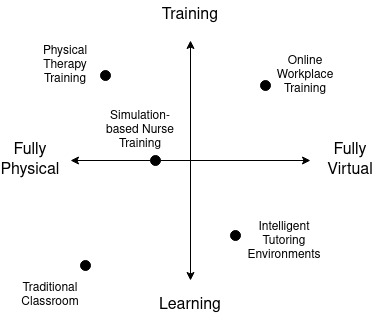
\includegraphics[width=0.4\textwidth]{img/LearningTrainingContinuum.jpg}
    \end{center}
    \caption{Learning-Training Continuum}
    \label{fig:ltcontinuum}
\end{wrapfigure}

% \begin{figure}
%     \centering
%     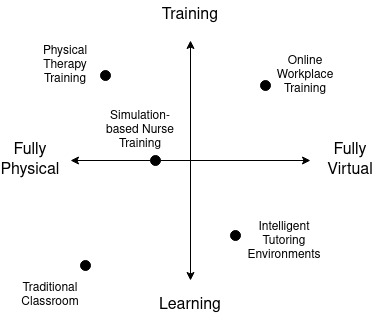
\includegraphics[width=0.5\textwidth]{img/LearningTrainingContinuum.jpg}
%     \caption{Learning-Training Continuum}
%     \label{fig:ltcontinuum}
% \end{figure}

One important aspect when considering the literature surrounding MMLA is identifying the contexts in which these techniques are used, which mostly fall under the category continuum of learning and training (see Figure \ref{fig:ltcontinuum}). The main goals of learning environments are education and knowledge gain. These venues range from conventional classrooms to online courses and self-paced learning environments. When we categorize these environments on our continuum shown in Figure \ref{fig:ltcontinuum}, we add a second dimension, between fully physical and fully virtual, to represent this wide range of learning environments. MMLA methods applied in learning environments focus on extracting insights from various modalities such as text, audio, video, and interactions to assess students' comprehension, engagement, and progress. Educators may modify instructional tactics, spot problematic students, and improve learning materials by analyzing these multimodal signals since they provide significant insights into both individual and group learning patterns.

On the other hand, training environments are designed to improve performance and build skills. This category encompasses professional training programs, simulations, and vocational training platforms, across the same potential continuum of fully virtual to fully physical that we use to categorize learning environments. In training settings, MMLA approaches are used to evaluate data in order to track the mastery of new skills, the accomplishment of tasks, and overall performance. These insights help instructors and managers adjust training programs, spot competency gaps, and determine how prepared students are for issues in the real world. The objectives of MMLA differ in learning and training situations, calling for specific strategies that take into account the specifics of each situation, but in this paper we review literature across the spectrum of learning and training.

However, it is important to note that this division isn't always clear-cut. Some environments of study, like those populated by PhD students, blur the line between education and training. PhD students are learning new things in a vein similar to learning environments, but they are also increasing their research abilities and expertise in a vein similar to a training program. Similarly, certain contexts, like game-playing platforms, defy easy classification into the learning or training categories. In these instances, MMLA methodologies must be flexibly applied, appreciating the multifaceted nature of the objectives at hand. In our categorization of all of the environments from our corpus of papers, we recognize this ambiguity in discrete categorization, but also recognize the utility of such a categorization when analyzing the research subcommunities that make up the larger field of MMLA. As such, we perform a fuzzy qualitative discrete categorization based on discussions among the authors of where we believe each paper’s environment best fits on our continuum shown in Figure \ref{fig:ltcontinuum}.

\subsubsection{Data Collection Mediums} \label{subsec:data_collection_mediums}
% Definitions reminders
% Researcher artifacts includes field notes and also labeling of the data (i.e., manual coding). 
% Participant artifacts includes pre/post tests and the like. To qualify, all artifacts must be collected and analyzed in the pipeline and cannot be collected post hoc afterward.
% Depth camera versus regular: discuss that both are video, but depth usually used for motion modality with skeletal features
% motion capture (posyx, accelerometer, gyroscope, magnetometer)
% Make point that things like learning gains and performance can fall into multiple categories depending on where derived from, e.g., logs, surveys, student artifacts (which can also be demo information)

The intricacies of learning gains and performance metrics underscore the diversity of sources within learning and training analytics frameworks, ranging from logs and surveys to student artifacts. A diverse range of data collection mediums plays a pivotal role in capturing a holistic picture of learners' progress, interactions, and struggles within educational and training environments. The mediums enumerated in Table \ref{tab:data_collection_mediums} (and all definitions in this section, for that matter) were identified through our qualitative analysis of the corpus.

\begin{table}[ht]
  \centering
  \caption{Definitions for Data Collection Mediums}
  \begin{tabular}{|c|p{0.8\textwidth}|}
    \hline
    \textbf{Medium} & \textbf{Definition} \\
    \hline
    VID & Sequence of video frames from a camera source. \\
    \hline
    AUD & Audio signals captured and converted by a microphone. \\
    \hline
    SCREEN & Sequence of video frames of the contents displayed on a device screen. \\
    \hline
    EYE & Eye movement data and gaze points captured by tracking devices with sensors and cameras. \\
    \hline
    LOGS & Environment logs containing data on participants' activities and interactions within the system. \\
    \hline
    SENSOR & Specialized sensors used to gather participants' physiological data. \\
    \hline
    INTER & Structured or unstructured conversations between researchers and participants. \\
    \hline
    SURVEY & Standardized sets of questions administered to participants. \\
    \hline
    PPA & (Participant Produced Artifacts). Materials produced by research participants using various mediums. This can include things like physical objects created for an engineering task or written responses to formative assessment questions. \\
    \hline
    RPA & (Researcher Produced Artifacts). Materials produced by the researchers that contribute to analysis and findings. This can include things like researchers' observational notes. \\
    \hline
    MOTION & Raw motion data collected by different devices/technologies. \\
    \hline
    TEXT & Raw textual input. \\
    \hline
  \end{tabular}
  \label{tab:data_collection_mediums}
\end{table}

In the context of video data, a distinction arises between depth cameras and traditional cameras. While both fall under the video medium, depth cameras are typically employed with the motion modality to emphasize skeletal features. Furthermore, within the Motion medium, the scope extends beyond general video data, encompassing technologies such as real-time location systems (RTLS) (e.g., accelerometers, gyroscopes, or magnetometers). These technologies offer diverse approaches to capturing raw motion data, providing granularity in understanding participants' physical movements.

Researcher Produced Artifacts (RPA) can range from detailed field observation notes capturing contextual nuances to labeling of data, often involving manual coding processes that enhance data interpretability and contribute to more nuanced analyses and findings. Similarly, Participant Produced Artifacts (PPA) constitute a valuable dimension in capturing participants' engagement and comprehension. These artifacts include a spectrum of materials, such as physical objects crafted by participants or the results of pre/post tests. Notably, to qualify as PPA, all artifacts must undergo collection within the designated research pipeline, excluding the collection of artifacts post hoc. 

\subsubsection{Modalities} \label{sec:modalities}
% Definitions

We identified several modalities used for analyzing and understanding participants' interactions with and within learning and training environments, as shown in Table \ref{tab:modalities}. 

\begin{table}[ht]
  \centering
  \caption{Definitions for Modalities}
  \begin{tabular}{|c|p{0.8\textwidth}|}
    \hline
    \textbf{Modality} & \textbf{Description} \\
    \hline
    AFFECT & The emotional state or affect exhibited by the participant. \\
    \hline
    POSE & The physical position, geolocation, or body posture of the participant. \\
    \hline
    GEST & The gestures and body language displayed by the participant. \\
    \hline
    ACT & The observable actions or activities performed by the participant. \\
    \hline
    PROS & Prosodic speech information, including volume, pauses, intonation, etc. \\
    \hline
    TRANS & Textual speech obtained through transcription, i.e., speech-to-text. \\
    \hline
    QUAL & Qualitative researcher observations on the participant's behavior or environment. \\
    \hline
    LOGS & Data related to the research context and participant's actions within the system. \\
    \hline
    GAZE & Data on the direction and focus of the participant's eye gaze. \\
    \hline
    INTER & Notes from interviews between researchers and participants. \\
    \hline
    SURVEY & Responses to surveys/questionnaires provided by the participant. \\
    \hline
    PULSE & The participant's pulse, indicating their heart rate. \\
    \hline
    EDA & Participant's electrodermal activity, measuring skin conductance as an indicator of arousal. \\
    \hline
    TEMP & Participant’s body temperature. \\
    \hline
    BP & Participant’s blood pressure. \\
    \hline
    EEG & Participant's electroencephalography activity, recording the brain's electrical signals. \\
    \hline
    FATIG & The level of fatigue experienced by the participant during the activity. \\
    \hline
    EMG & Participant's electromyography activity, measuring muscles' electrical signals \\
    \hline
    PPA & (Participant Artifacts). Artifacts produced by the participant. \\
    \hline
    RPA & (Researcher Artifacts). Artifacts produced by the researcher. \\
    \hline
    SPECT & (Audio Spectrogram). Visual representation of audio frequencies in the form of a spectrogram. \\
    \hline
    TEXT & Raw text data generated by the participant in the study environment. \\
    \hline
    PIXEL & Raw RGB pixel values representing visual information captured by cameras or sensors. \\
    \hline
  \end{tabular}
  \label{tab:modalities}
\end{table}

In the context of a modality as a unique attribute defined by data from one or more data streams, it is important to note that multimodality can arise from a combination of either multiple modalities or multiple data streams. For example, the same video data stream could be used to derive both the AFFECT and POSE modalities. %demonstrating how a single source can contribute to distinct attributes. 
Similarly, the AFFECT modality could be derived from separate audio and video datastreams. %exemplifying how information from different sources can collectively form a multimodal perspective.

\subsubsection{Analysis Methods} \label{subsec:analyis_methods}
% Definitions
% Pattern extraction analysis usually refers to identifying sequences, but can be other types of patterns (include examples, revisit later). Used as catch-all for when patterns are identified but do not fall under other subsets of pattern extraction like clustering. Sequwnce mining, some HMM applications, etc.
% Define classification for our purposes as using an algorithm to predict an output in a discrete space. Mention RL paper as using RL but falling into classification category by our definition. 
% Add caveat that analysis methods refers to analysis only of the data and not of the actual analysis, unless analysis of the analysis provides more information about the data (show examples)

The classification scheme outlined in Table \ref{tab:analysis_methods} was developed with the intent of identifying the prevalent analysis methods employed in the diverse landscape of multimodal learning and training environments. The presented analysis methods, ranging from supervised tasks like Classification (CLS) to unsupervised techniques such as Clustering (CLUST), reflect the rich variety of strategies employed in the field. Evaluating these methods is imperative within the context of this review, as they offer insights into the prevailing analysis trends in the field and help guide future research directions.

\begin{table}[ht]
\centering
\caption{Definitions of Analysis Methods}
\begin{tabular}{|l|p{0.82\textwidth}|}
\hline
\textbf{Abbreviation} & \textbf{Definition} \\
\hline
CLS & Classification is a supervised learning task in machine learning where the goal is to assign labels or categories to input data based on its features. It involves training a model on a labeled dataset to learn the mapping between input features and their corresponding output labels, enabling the model to make predictions on new, unseen data. \\
\hline
REG & Regression is a supervised learning task that focuses on predicting continuous numerical values. In contrast to classification, where the output is categorical, regression involves training a model to understand the relationships between input features and continuous target values, allowing for the prediction of numerical outcomes. \\
\hline
CLUST & Clustering is an unsupervised learning technique that involves grouping similar data points together based on their inherent patterns or similarities. Unlike classification, clustering does not rely on predefined labels, and the goal is to discover hidden structures within the data, grouping similar observations into clusters. \\
\hline
QUAL & Qualitative analysis involves the examination and interpretation of non-numerical data, often in the form of textual or visual information. It aims to uncover patterns, themes, or meanings within the data that is rich and context-dependent. \\
\hline
STATS & Statistical methods encompass a broad range of techniques used to analyze data and draw meaningful conclusions. This includes descriptive statistics (such as mean, median, and standard deviation) and inferential statistics (such as hypothesis testing, ANOVA, and correlation), which help researchers make inferences about generalizability based on sample data. \\
\hline
NET & Network analysis involves the study of relationships and interactions among entities in a network. It includes graph-based approaches where nodes represent entities (e.g., individuals, concepts) and edges represent relationships or connections between them.  \\
\hline
PATT & Pattern extraction refers to the process of identifying meaningful patterns or structures within data. This can include various techniques such as Markov analysis and sequence mining, where patterns in the temporal order of events are discovered, or other methods aimed at uncovering hidden structures that provide insights into the underlying dynamics of the data. \\
\hline
\end{tabular}
\label{tab:analysis_methods}
\end{table}

\subsubsection{Data Fusion} \label{subsec:data_fusion}
% Graphic with different kinds of fusion
% Fusion definitions:
%   Early fusion. Raw, obserable data is fused directly from data collection medium and used for analysis. E.g. using raw audio signal and screen pixels, and fusing them for analysis.
%   Mid fusion. Observable features are unimodally extracted from raw data, and those extracted features are fused for analysis. E.g. extract affect from video and transcriptions from speech and fusing them for analysis. 
%   Add that we consider "cognitive load" an "observable" feature, as it comes out-of-the-box with some sensors' software (e.g. Kinect)
%   Late fusion. Unobservable features are extracted from the data, and then fused for analysis. E.g., fusing neural network output for analysis.
%   Explain: None or Other (OTH) fusion, hybrid fusion
%       cite Chango: A review on data fusion in multimodal learning analytics and educational data mining
%       "studies that do not fit into none of those three groups or in which the fusion point was not specified (Others category)"
%   Hybrid can either be separate pipelines (as traditionally defined) or multiple data types in the same pipeline

%   di mitri paper reference for observable/unobservable fusion definition: https://onlinelibrary.wiley.com/doi/full/10.1111/jcal.12288

In the realm of multimodal learning learning and training, data fusion plays a pivotal role in harnessing the power of multiple data sources to provide a more comprehensive and insightful understanding of the learning process. The process of data fusion involves combining information from various sources to create a unified dataset, thereby facilitating enhanced interpretation and analysis relative to analyzing only a single modality at a time. By combining data from multiple modalities, researchers and educators can uncover hidden insights into learners' cognitive states, emotions, and behaviors. This comprehensive understanding paves the way for personalized interventions and more effective pedagogical strategies. 

Within data fusion, the traditional method of categorization, as underscored by Chango et al.’s \cite{Chango2022} recent review of data fusion within MMLA, is based on three categories: early, late, and hybrid. The \textit{early fusion} approach involves combining raw data from multiple sources at the earliest stage of processing. This integration occurs before any individual modality-specific analysis, allowing for joint processing of data from different sources. By merging information early, the model can capture potential interactions and dependencies among modalities, but is limited by cases where there are significant differences between data modalities and challenges surrounding the complexity and explainability of the joint modality models. The \textit{late fusion} approach involves performing separate analyses on individual modalities and then integrating their outcomes at a later stage. This method allows for specialized processing of each modality's characteristics, potentially leading to more accurate and contextually relevant insights, but is limited in its ability to capture intermodal relationships that might exist. The \textit{hybrid fusion} approach aims to combine the strengths of both early and late fusion methods. In this approach, data from various sources are combined at multiple stages of processing. For instance, an initial early fusion step might be followed by separate analyses of each modality using a late fusion strategy. This allows for the exploitation of intermodal relationships while also accommodating the uniqueness of each modality's information. However, hybrid models increase the overall complexity of data analysis and require a priori decisions about which features should be combined at what points in the model pipeline. The choice of fusion method depends on several factors, including the specific problem domain, the characteristics of the available data, the desired level of interpretability, and the computational resources available.

However, we argue that this traditional three-state categorization is actually not informed enough to fully capture the complexity of multimodal analysis. After a qualitative review of our corpus, we encountered considerable difficulty categorizing analysis methods into just these three categories due to the ambiguity surrounding what constitutes \textit{raw features} compared to \textit{processed features}. For example, some researchers might classify the joint position data measured by a Microsoft Kinect camera as a raw feature, and thus permissible in early fusion, since it is available from the camera without any additional processing by the researchers. However, others might classify this as a processed feature, and thus a part of hybrid or late fusion, since the Kinect camera is actually computing this data from the raw depth data, regardless of whether this computation is obfuscated to the end user. Qualitatively, we noticed this pattern and disagreement among researchers with multiple modalities within our paper corpus. Motivated by this finding, we propose an additional category of data fusion, which we call \textit{mid fusion}. 

Mid-fusion represents a middle point between early fusion and late fusion, where data could be somewhat processed and transformed before being combined, but not transformed to the same extent as in late fusion. The difference here between mid and late fusion can be somewhat subtle depending on the modality, but is perhaps best explained using Di Mitri et al.’s \cite{DiMitri2018} conceptualization of the \textit{observability line}. In their work, modalities are categorized into \textit{input space}, which represents observable evidence and data that can be tracked with sensors, and \textit{hypothesis space}, which represents inferred learning labels. These two categories are separated by the \textit{observability line}, which they describe as "a line of separation between the observable evidence and all the possible interpretations" \cite{DiMitri2018}. In our new framework for categorizing data fusion, \textit{early fusion} represents combining features without any initial processing, \textit{mid fusion} represents combining features that have had prior processing but stay within the input space (i.e., they are still observable features), and \textit{late fusion} represents combining features that have had prior processing that crosses the observability line into the hypothesis space (i.e., they are no longer directly observable).

For example, consider the same Kinect sensor discussed earlier. In this case, the raw pixel values from the camera image or the raw depth values from the depth sensor would be considered unprocessed, observable features and candidates for early fusion. However, the joint position coordinates output by the camera SDK would be considered observable, processed features, and thus candidates for mid fusion, since they are derived from other observable data but still remain directly observable. Beyond this, if a researcher used the joint position data as input to another model which estimated a measure of motivation, for example, then this motivation construct would only be a candidate for late fusion, since we have now crossed the observability line. 

This classification is still somewhat qualitative and up to a researcher's interpretation. As described by Di Mitri et al., "The distinction between observable/unobservable is conceptual and can vary in practice." \cite{DiMitri2018}; however, we believe that this additional data fusion category helps to resolve some of the ambiguity related to the original categorization scheme and is useful for identifying the sub-communities of multimodal learning and training based on which methods researchers have applied. For a concrete definition of the modalities that we consider observable for the categorization in this paper, see section \ref{sec:modalities}. In addition to the early, mid, late, and hybrid data fusion categories, in this paper, following the methodology of Chango et al. \cite{Chango2022}, we add an \textit{other} category to catch studies that do not fit into one of those four groups or in which the fusion point was not specified (or fusion was not performed).

\subsubsection{Environment Setting} \label{subsec:environment_setting}
% Confirm exact set from S18 corpus to be sure!
% Environment Setting. Physical, virtual, blended, unspecified.

Analyzing the contextual settings in which these studies unfold, we categorize the learning and training environments as: %, as shown in Table \ref{tab:environment-settings}

\begin{itemize}
    \item \textbf{Virtual (VIRT)}: Learning or training activities take place entirely within a virtual space, such as when participants engage with content and exercises within a computer-based system.  
    \item \textbf{Physical (PHYS):} Activities unfold in a physical, real-world environment. This includes traditional classroom settings and other tangible spaces where learning or training occurs without reliance on digital technologies. 
    \item \textbf{Blended (BLND):} Learning or training activities blend elements of both the virtual and physical realms. Environments characterized by augmented reality, mixed reality, or a combination of digital and physical components fall into this category. 
    \item \textbf{Unspecified (UNSP):} Designated when the papers analyzed do not provide sufficient information about a study's learning environment to be conclusively categorized.    
\end{itemize}

The reasons for analyzing the environmental settings are twofold. First, we aim to unveil the contextual relevance of multimodal learning and training, discerning how these approaches manifest in computer-based (virtual) spaces, traditional classrooms (and other physical environments), and blended scenarios combining virtual and physical elements. Additionally, our categorization acknowledges instances where information about the environment setting is not sufficiently provided, directing attention to research gaps and unexplored areas within the current literature.

% Joyce: is a table better?
% \begin{table}[h]
%   \centering
%   \caption{Definitions for Environment Settings}
%   \label{tab:environment-settings}
%   \begin{tabular}{|c|p{0.85\textwidth}|}
%     \hline
%     \textbf{Setting} & \textbf{Definition} \\
%     \hline
%     Virtual & Learning or training activities take place entirely within a virtual space, such as when participants engage with content and exercises within a computer-based system. \\
%     \hline
%     Physical & Activities unfold in a physical real-world environment. This could encompass traditional classroom settings or any other tangible space where learning or training occurs without reliance on digital technologies. \\
%     \hline
%     Blended & Learning or training activities blends elements of both the virtual and physical realms. Environments characterized by augmented reality, mixed reality, or a combination of digital and physical components fall into this category. \\
%     \hline
%     Unspecified & Designated when the papers analyzed do not provide sufficient information about the setting to be conclusively categorized. \\
%     \hline
%   \end{tabular}
% \end{table}


\subsubsection{Environment Subject} \label{subsec:environment_subject}
% Confirm exact set from S18 corpus to be sure!
% Environment Subject. STEM, humanities, psychomotor skills, other, unspecified

While conducting our analysis, we recognized the importance of identifying the subject matter domains that study participants were engaged in during their educational and training experiences. This categorization not only further helps contextualize the application of multimodal learning and training analytics, but also allows for dynamically exploring how these methods intersect with a diverse array of domains. To systematize this classification, we identified five subject matter categories, which are listed below. These categories are intentionally broad, as we observed that introducing additional granularity %would not substantially contribute to a better understanding the current trends in the field of multimodal learning analytics applied to learning and training environments.
% , defined in Table \ref{tab:environment-subjects}: STEM, Humanities, Psychomotor Skills, Other, and Unspecified.  
hindered our ability to analyze and understand the current trends in the field due to the corpus's widely varied subject matter.
\begin{itemize}
    \item \textbf{STEM:} Participants engaged in learning or training related to Science, Technology, Engineering, and Mathematics (STEM) disciplines. In our case, this also includes applied scientific disciplines such as healthcare and medicine.
    \item \textbf{Humanities (HUM):} Participant activities focused on disciplines such as literature, debate, oral presentation, and other humanities-related fields.
    \item \textbf{Psychomotor Skills (PSY):}  Learning or training activities emphasizing the development of motor skills and coordination.
    \item \textbf{Other (OTH):} Subjects that do not fall into the above categories. This could encompass a wide range of topics beyond STEM, humanities, or psychomotor skills.
    \item \textbf{Unspecified (UNSP):} Designated when the papers analyzed did not provide sufficient information about the subject matter to be conclusively categorized.
\end{itemize}

Importantly, papers reporting results from multiple studies are categorized with labels corresponding to the environment subject of each study \cite{3796643912,2055153191}. 


%Joyce: would a table be better?
% \begin{table}[ht]
%   \centering
%   \caption{Definitions for Environment Subjects}
%   \label{tab:environment-subjects}
%   \begin{tabular}{|c|p{0.78\textwidth}|}
%     \hline
%     \textbf{Subject} & \textbf{Definition} \\
%     \hline
%     STEM & Participants engaged in learning or training related to Science, Technology, Engineering, and Mathematics (STEM) disciplines. \\
%     \hline
%     Humanities & Participant activities focused on disciplines such as literature and other humanities-related fields. \\
%     \hline
%     Psychomotor Skills & Learning or training activities emphasizing the development of motor skills and coordination. \\
%     \hline
%     Other & Subjects that do not fall into the above categories. This could encompass a wide range of topics beyond STEM, humanities, or psychomotor skills. \\
%     \hline
%     Unspecified & Designated when the papers analyzed do not provide sufficient information about the subjects to be conclusively categorized. \\
%     \hline
%   \end{tabular}
% \end{table}




\subsubsection{Participant Structure} \label{subsec:participant_structure}
% Confirm exact set from S18 corpus to be sure! 
% Participant Structure. Individual, multi-person

% Joyce: there are no unspecified paper in the corpus
% Clayton: awesome thanks for pointing this out!

We categorized papers' participant structures based on whether the analysis of the studies focused primarily on individual or multi-person learning and training experiences. The classification comprises two primary categories: 
\begin{itemize}
    \item \textbf{Individual (IND)}: Environments where learning or training activities center around individual participants.
    \item \textbf{Multi-Person (MULTI)}: Environments where learning or training activities involve multiple participants, often emphasizing collaborative or group dynamics. 
\end{itemize}

It's noteworthy that some papers analyzed both types of environments, reflecting the diversity in studies even within individual publications \cite{1326191931, 3637456466}. This categorization illuminates the varying scopes of analysis focus, shedding light on instances where multimodal analytics are tailored to individual learners and others where collaborative (and other multi-person) learning and training experiences take precedence.

\subsubsection{Didactic Nature} \label{subsec:didactic_nature}
% Didactic Nature. Instructional, training, informal, unspecified 
% Joyce: confirmed on S18

Didactic nature refers to the ``type" of learning or training that transpires in each study's environment, which we use as yet another lens through which to understand, analyze, and differentiate learning and training environments. Our categorization scheme comprises 4 distinct categories:

\begin{itemize}
    \item \textbf{Instructional (INSTR)}: Studies where the primary focus is on formal instruction, including traditional classroom settings, online courses, or any structured learning environment with clear instructional objectives.

    \item \textbf{Training (TRAIN)}: Studies categorized under TRAIN emphasize skill development, practical training, or professional development. This involves scenarios where participants are acquiring specific skills or competencies relevant to their profession or field.
    
    \item \textbf{Informal (INF)}: Informal environments involve learning or training that occurs in a more unstructured manner, outside formal instructional or training environments. For instance, \citet{666050348} aimed to bridge multimodal interaction to the game Minecraft\footnote{https://www.minecraft.net/en-us} to support diverse learners in non-traditional learning environments. 
    
    \item \textbf{Unspecified (UNSP)}: This category is applied when the papers do not provide sufficient information about the didactic nature of the study. It acknowledges instances where the training or educational context is not clearly defined or detailed in the literature.
\end{itemize}

\subsubsection{Level of Instruction or Training} \label{subsec:level_of_instruction}
% Confirm exact set from S18 corpus to be sure! Joyce: confirmed
% Level of Instruction or Training. K-12, university, professional development
We sought to delineate the level of instruction or training for participants, providing valuable insights into the educational contexts targeted by these analyses. The following categories capture the diverse training and educational levels represented in our survey:

\begin{itemize}
    \item \textbf{K-12}: Participants at the primary or secondary education levels, encompassing kindergarten through 12th grade.
    \item \textbf{University (UNI)}: Participants engaged in university-level education, including both undergraduate and graduate students.
    \item \textbf{Professional Development (PROF)}: Participants involved in training or learning experiences specifically designed for professional development and not tied to a K-12 or university curriculum.
    \item \textbf{Unspecified (UNSP)}: Designated when papers did not provide sufficient information about the participants' level of instruction or training.
\end{itemize}

It is important to note that studies featuring multiple groups of participants, or those reporting results across various studies, may have been assigned multiple labels, reflecting the diversity inherent to the set of papers in our corpus.

\subsubsection{Analysis Approach} \label{subsec:analysis_approach}
% MB vs MF.

While the analysis methods exhibited significant variability, we systematically categorized the overarching analysis approaches into two main categories: \textbf{model-based} and \textbf{model-free}.

Model-based analysis involves constructing a formal representation, or model, to elucidate the underlying structure of the data. These models are built based on predefined assumptions about the relationships within the data. For example, in machine learning applications, a model-based approach may entail creating mathematical functions that capture the relationships between input features and output labels. In the broader context of cyber-physical systems, model-based analysis may involve developing computational models that represent the dynamics of the system and its interactions.

On the other hand, model-free analysis refers to approaches that do not explicitly construct a model of the underlying data distribution or predict outcomes. Instead, these methods directly learn patterns and relationships from the data without assuming a specific form defined by an underlying model. 

It is noteworthy that the categorization of papers into model-based or model-free analysis approaches is not mutually exclusive. It is multi-label, signifying that a single paper may receive both labels if it reports the utilization of different analysis approaches within the same paper. 

\section{Methods} \label{sec:methods}

% Overview of methods section to include lit search, study selection, feature extraction, and analysis methods

This section details the methods used to construct our literature corpus and the efforts taken to consider all relevant papers, which we then distill via both quantitative (graph-based) and qualitative (quality control) methods to a manageable amount of works we believe to be representative of the current state of the field. In doing so, we introduce a novel, graph-based literature review corpus reduction procedure that uses a directed citation graph to exclude irrelevant works based on a paper's incoming and outgoing citations. We call our approach \textit{citation graph pruning} (CGP), which we discuss in Section \ref{subsubsec:cgp}. To the authors' knowledge, this approach has not been previously used for distilling a literature review corpus. Our procedure for performing the quality control portion of this literature review is adapted from Barbara Kitchenham's ``Procedures for Performing Systematic Reviews" \cite{kitchenham2004procedures}.

\subsection{Literature Search} \label{subsec:literature_search}

Our literature search consists of 42 queries defined, discussed, and agreed upon by the authors as being representative of the body of works this literature review would be conducted on. Instead of performing our queries manually, we opted to perform our queries programmatically via an API-based Google Scholar web scraping tool. There are several available tools for scraping Google Scholar, such as scholarly\footnote{\href{https://pypi.org/project/scholarly/}{https://pypi.org/project/scholarly/}} and gscholar\footnote{\href{https://github.com/venthur/gscholar}{https://github.com/venthur/gscholar}}. Ultimately, we employed SerpAPI\footnote{\href{https://serpapi.com/google-scholar-api}{https://serpapi.com/google-scholar-api}}, a third-party Google Scholar web scraping API, for its most essential feature: organic web results. Other API tools' results are not organic, i.e., a query made via the API and one manually queried in a browser-based environment will produce two different sets of results.

Queries were posed via API request to Google Scholar for papers published between 1/1/2017 and 10/22/2022 (the date of our literature search). 2017 was collectively agreed upon as being the best cutoff date for inclusion in our search due to the rapid technological advancements in the field over the past 5 years. Several papers prior to 2017 are discussed in Section \ref{sec:intro_background}, as they are seminal works; however, they are not considered for inclusion in our corpus. 

For the literature search, this review's authors decided on 14 distinct search strings, and each string was searched 3 times with a different spelling of the word \textit{multimodal} --- multimodal, multi-modal, and multi modal --- prepended to it. The 14 search strings are enumerated in Table \ref{tab:search_terms}\footnote{The term ``xai" was originally included in the search queries due to the authors' interest in exploring explainable AI methods applied to learning and training environments. Unfortunately, the field is still nascent, and no usable query results were returned given our search criteria.}.

\begin{table}[htbp]
    \renewcommand{\arraystretch}{1.3}%
    \centering
    \caption{Search strings used for the literature search.}
    \begin{tabularx}{\linewidth}{l@{\hskip .25in} l@{\hskip .25in}}
    
        \midrule
        education technology & explainable artificial intelligence \\

        \midrule
        learning analytics & learning environments \\
        
        \midrule
        learning environments literature review & learning environments survey \\
    
        \midrule
        literature review & simulation environments \\
        
        \midrule
        survey & training environments \\
        
        \midrule
        training environments literature review & training environments survey \\
        
        \midrule
        tutoring systems & xai \\

        \bottomrule
    \end{tabularx}
    \label{tab:search_terms}
\end{table}

For each of the 42 queries, the top 5 pages (100 publications) deemed most relevant by Google Scholar were collected. The top-5 cutoff was financially imposed because of our subsequent citation graph construction (see Section \ref{subsubsec:cgp}). To build the citation graph, each individual paper's citation information is queried, but each query is capped at 20 citations per API call by SerpAPI. This means that a paper with 100 citations requires 5 additional API calls to gather all of its citation information. The number of API calls needed to construct the citation graph would be intractable (and unaffordable) if the initial search was left unbounded; therefore, the top-5 cutoff was put in place.

Our initial search yielded a total of 4,200 papers (14 unique search terms * 3 spellings of multimodal * 100 publications per query). The distillation procedure we used for corpus reduction is enumerated in Table \ref{tab:procedure} and discussed in the following subsections. Throughout this section, each step of our corpus reduction procedure is identified via its Step ID in Table \ref{tab:procedure}.

\begin{table}[htbp]
    \renewcommand{\arraystretch}{1.3}%
    \centering
    \caption{Our corpus reduction procedure. Step ID 0 is the literature search. Steps 1 and 2 used programmatic filtering via Python packages. Steps 3-5 were performed quantitatively via CGP. Step 6 uses regex filtering via a human-in-the-loop. Steps 7-9 were performed qualitatively via our quality control procedures. At each step of the corpus reduction procedure, the number of papers pruned and number of papers remaining are listed.}
    \begin{tabularx}{\linewidth}{l@{\hskip .25in} l@{\hskip .25in} l@{\hskip .25in} l@{\hskip .25in}}
        Step ID & Procedure & Removed & Remaining \\
        \midrule
        
        0 & Literature search & 0 & 4200\\
        
        1 & Remove duplicates & 2079 & 2121\\

        2 & Remove non-English & 1 & 2120\\

        3 & Remove degree-0 nodes & 488 & 1632\\
        
        4 & Remove disconnected components & 101 & 1531\\
        
        5 & Iteratively remove degree-0 and degree-1 nodes & &\\

        \quad 5.1 & \quad Iteration 1 & 373 & 1158\\

        \quad 5.2 & \quad Iteration 2 & 74 & 1084\\
        
        \quad 5.3 & \quad Iteration 3 & 19 & 1065\\
        
        \quad 5.4 & \quad Iteration 4 & 2 & 1063\\

        6 & Remove titles with keywords & 204 & 859\\
        
        7 & Title reads & 471 & 388\\
    
        8 & Abstract reads & &\\
        \quad 8.1 & \quad Remove inaccessible abstracts & 10 & 378\\
        \quad 8.2 & \quad First abstract round & 211 & 167\\
        \quad 8.3 & \quad Second abstract round & 40 & 127\\

        9 & Full paper reads & & \\
        \quad 9.1 & \quad First full paper round & 52 & 75\\
        \quad 9.2 & \quad Feature discretization and extraction & 2 & 73\\
        \quad 9.3 & \quad Second full paper round & 0 & 73\\
        \quad 9.4 & \quad Second feature extraction round & 0 & 73\\
        \bottomrule
    \end{tabularx}
    \label{tab:procedure}
\end{table}

Our initial corpus contained 2,079 duplicates, which were removed by hashing paper titles (Table \ref{tab:procedure}, Step ID 1). If a paper had multiple versions (or other duplicates), we used the official source (e.g., journal or conference) of publication. We removed 1 non-English paper (Table \ref{tab:procedure}, Step ID 2) due to pragmatism (English is the only language shared between all of this review's authors). Non-English papers were identified using spaCy FastLang\footnote{\href{https://spacy.io/universe/project/spacy_fastlang}{https://spacy.io/universe/project/spacy\_fastlang}}, where any paper whose title was identified as having less than a 100\% chance of being English was selected for manual review and potential exclusion. In total, our initial search yielded 2,120 unique (English) papers published during or after 2017.

\subsection{Study Selection} \label{subsec:study_selection}
To reduce our corpus to a reviewable body of works, we employed both quantitative ans qualitative methods. After the initial search, we distilled the corpus quantitatively via CGP, which we discuss in Section \ref{subsubsec:cgp}. Subsequent distillation was performed via qualitative means and is discussed in Section \ref{subsubsec:quality_control}. 

\subsubsection{Citation Graph Pruning (Quantitative Corpus Reduction).}\label{subsubsec:cgp}

For visualization, analysis, and distillation purposes, we used \href{https://networkx.org/}{NetworkX} to create and display a \textit{citation graph} of the initial 2,120 works considered for inclusion in this review. The citation graph is a directed acyclic graph (DAG), where each node is a paper uniquely identifiable by its UUID (universally unique identifier) on Google Scholar, and each directed edge from A to B indicates paper A cites paper B. For the purposes of this paper, we consider the degree of each node (paper) $p$ to be the sum of both incoming and outgoing edges, i.e., papers citing $p$ and papers cited by $p$, respectively. We again used SerpAPI for collecting the list of works that cited each paper. The citation search did not need to be conducted in both directions, as any paper citing another paper in our corpus would already have been identified by the ``cited by" list of the paper being cited. Citations by papers not included in our initial search (i.e., in the DAG) were ignored. Initially, our DAG contained a 3-node cycle. This was due to preprint overlap, as papers by the same author cited each other while in progress. Once the cycle was identified, its nodes' edges were updated, and the cycle was removed. No nodes were removed as a result of correcting the cycle.

Once the DAG was constructed, we removed all 0-degree nodes (Table \ref{tab:procedure}, Step ID 3) (i.e. nodes with no edges coming in or going out). We felt it reasonable that if a paper did not cite (or was not cited by) any other papers in the field as determined by our literature search, then the paper was either not relevant to the field or did not yield methods or findings referenced by subsequent works. Importantly, our approach strikes a balance between incoming and outgoing citations, as earlier works are unable to \textit{cite} many works in the corpus, and later works are unable to \textit{be cited by} many works in the corpus. For example, works from early 2017 may not have any outgoing edges simply due to being some of the earliest works in the corpus, which would have prevented them from citing papers that had not yet been published. However, these same papers had a greater opportunity to be cited by subsequent papers, which is why we felt it important to consider both incoming and outgoing edges: we expect earlier papers to have more incoming edges and later papers to have more outgoing edges. Altogether, pruning 0-degree nodes from the DAG reduced our corpus by 488, dropping our count to 1,632 works.

After removing 0-degree nodes, we examined the DAG's connectivity (Table \ref{tab:procedure}, Step ID 4) to identify disconnected components not relevant to our literature search. This had to be done to account for overlapping terminology across domains. For example, a cursory look at our initial search results included several ``multimodal training" papers related to deep learning (DL), where artificial neural networks (ANNs) are trained using data across multiple modalities but are not applied to multimodal learning or training environments. Our hypothesis, based on our search strings, was that the works relevant to this review would comprise the largest component of the DAG, leaving other smaller, disconnected components to be discarded as irrelevant because they lacked any edge to or from the DAG's primary component.

Evaluating the DAG's connectivity, we found one large component consisting of 1,531 nodes (papers) and 4 smaller, disconnected components of various sizes. The disconnected components totaled 101 papers. The sizes of the disconnected components, their frequencies of occurrence in the DAG, and the total number of papers for each component size are listed in Table \ref{tab:disconnected}. All 101 papers were removed from the corpus by pruning the DAG's disconnected components, which left 1,531 papers represented by a single, connected graph. 

\begin{table}[htbp]
    \renewcommand{\arraystretch}{1.3}%
    \centering
    \caption{Disconnected DAG components by number of nodes in the component (component size), frequency of occurrence, and total number of papers. For instance, the first row indicates that there were 35 disconnected components of size 2 in the graph, totaling to 70 papers.}
    \begin{tabularx}{0.5\linewidth}{l@{\hskip .25in} l@{\hskip .25in} l@{\hskip .25in}}
        Component Size & N Occurrences & Papers \\
        \midrule
        
        2    &  35 &  70\\
        \midrule
        
        3    &  6  &  18\\
        \midrule
        
        4    &  2  &  8\\
        \midrule
        
        5    &  1  &  5\\

        \bottomrule
    \end{tabularx}
    \label{tab:disconnected}
\end{table}

Once we had our connected graph, we removed 1-degree nodes to further prune it. This created new 0-degree nodes, which were also subsequently removed. This process of removing 1- and 0-degree nodes was repeated iteratively four times (Table \ref{tab:procedure}, Step ID 5) until the graph was stable (i.e., removing 1-degree nodes did not create any new 0-degree nodes). By iteratively removing 1- and 0-degree nodes, we felt we could effectively identify and remove works outside the scope of our literature review without losing works directly related to multimodal learning and training environments. This is because the field of multimodal learning and training environments spans several sub-fields across computer science, education, and cyberphysical systems, and the authors agreed it was unlikely papers with so few edges would be relevant to our review if they had not cited (or been cited by) more than a few other works in our corpus. We removed 373 nodes in the first iteration (Table \ref{tab:procedure}, Step ID 5.1), 74 nodes in the second iteration (Table \ref{tab:procedure}, Step ID 5.2), 19 nodes in the third iteration (Table \ref{tab:procedure}, Step ID 5.3), and 2 nodes in the fourth and final iteration (Table \ref{tab:procedure}, Step ID 5.4). Altogether, we removed 468 papers across four iterations, which reduced our corpus from 1,531 papers to 1,063. 

Manually examining the remaining 1,063 titles informed us that a large part of our corpus was still outside the scope of our review. First, we  noticed there were still many papers related to training multimodal neural networks. We also noticed many works applying multimodal methods to the medical field, usually in terms of medical imaging. To remove papers pertaining to multimodal neural network training and multimodal medical applications, we programmatically identified 217 titles via regex keyword search (Table \ref{tab:procedure}, Step ID 6) that contained at least one of the six following words: neural, deep, machine, medical, medicine, and healthcare. We then evaluated the selected titles by hand. Of the 217, 13 were kept in the corpus due to their potential relevance to our review. Papers employing deep learning methods in multimodal learning analytics (MMLA) and applying multimodal methods to medical learning or training environments were within the scope of our review, for example. As examples, we removed one paper titled, ``deep learning for object detection and scene perception in self-driving cars: survey, challenges, and open issues" \cite{gupta2021deep}; and we kept one titled, ``supervised machine learning in multimodal learning analytics for estimating success in project‐based learning" \cite{spikol2018supervised}. The remaining 204 papers were removed from the corpus, reducing it to 859 potentially relevant works.

It was at this point we concluded our quantitative pruning procedure and began qualitatively reducing the corpus, which we discuss in the next subsection.

\subsubsection{Quality Control (Qualitative Corpus Reduction).} \label{subsubsec:quality_control}

After applying quantitative methods to prune the corpus via CGP, we employed qualitative methods to further reduce the dataset by hand. This involved selecting papers for exclusion based on consensus. Pursuant to Kitchenham \cite{kitchenham2004procedures}, we initially excluded works based on reading papers' titles, then abstracts, and eventually full manuscripts. The first five authors of this review acted as reviewers for the quality control procedure. 

For the title reads (Table \ref{tab:procedure}, Step ID 7), four of the reviewers read all 859 titles. For each title, each reviewer independently determined whether the title was likely to fall inside the scope of the review. The results were tallied, and papers were then selected for inclusion/exclusion based on majority voting, i.e., papers with at least three votes ``for" were automatically included, and papers with at least three votes ``against" were automatically excluded. For the papers with a 2-2 tie, a fifth reviewer was used as a tie breaker. The reviewers selected 347 papers for inclusion and 372 papers for exclusion. 140 papers were tied, and a fifth reviewer selected 41 of those for inclusion. In total, 388 papers were selected for inclusion after the title reads --- 347 by majority vote, and 41 by tie-breaker.

Before conducting the abstract reads (Table \ref{tab:procedure}, Step ID 8), several works were excluded due to their inaccessibility (Table \ref{tab:procedure}, Step ID 8.1). While gathering the abstracts, we noticed not all papers were publicly available. Several were defined by invalid URLs or behind paywalls. Whenever a paper's abstract (or introduction, in the case of a book) was unavailable via its SerpAPI URL, a Google search was conducted in order to obtain the abstract manually through websites such as ResearchGate\footnote{\href{https://www.researchgate.net/}{https://www.researchgate.net/}} and other academic repositories. When this failed, we relied on the [Anonymous] University Library's proxy to access papers behind paywalls. If we were unable to freely access a paper's abstract online through Google search or via Vanderbilt's proxy, the paper was excluded from the corpus. Altogether, 10 papers were removed due to inaccessibility, leaving 378 papers for the abstract reads.

The ``abstracts" quality control procedure consisted of two rounds. Similar to the procedure for the title reads, each of the remaining 378 abstracts was first assigned to two reviewers, and a majority voting scheme was employed (Table \ref{tab:procedure}, Step ID 8.2). Papers were then selected for inclusion or exclusion based on a predefined set of exclusion criteria. The exclusion criteria for the abstracts is listed in Table \ref{tab:abstract_exclusion_criteria}. Exclusion criteria are cumulative, so each criterion applies to subsequent steps in our corpus reduction procedure. An exclusion criterion for the abstracts will similarly apply to full paper reads later on, for example.

\begin{table}[htbp]
    \renewcommand{\arraystretch}{1.3}%
    \centering
    \caption{Exclusion criteria for the abstract reads. Each of the 378 abstracts was assigned to two different reviewers. Each reviewer was instructed to exclude works based on this set of criteria.}
    \begin{tabularx}{\linewidth}{l@{\hskip .25in}}
        \midrule
        1. Paper does not deal with learning or training environments \\
        2. Paper's environment is VR-only \\
        3. Paper does not analyze multimodal data \\
        4. Paper does not apply multimodal analysis methods \\
        5. Paper is not original applied research\\
        \bottomrule
    \end{tabularx}
    \label{tab:abstract_exclusion_criteria}
\end{table}

Because this literature review focuses on multimodal methods applied to learning and training environments, any paper not dealing with a learning or training environment was not considered for this review. As mentioned in Section \ref{sec:intro_background}, VR environments were also not considered for inclusion in our corpus due to issues with scaling this technology in classroom settings and the lack of semantic meaning with respect to the environment for video analysis. If a paper does not analyze multimodal data, it is similarly out-of-scope for this review. Papers must also include systematic methods for analyzing the multimodal data, and those methods must be original, applied research. Papers that are literature reviews, pedagogical tools, theoretical foundations, doctoral consortiums, etc., may be used for reference in our Introduction and Background, but they are not considered for inclusion in the actual review corpus unless they additionally provide original, applied research via multimodal methods and analysis.

Of the 378 abstracts, reviewers agreed to keep 96 papers (i.e., both reviewers selected the work for inclusion) and discard 211 (i.e., both reviewers selected the work for exclusion). 71 were selected for further review (i.e., one reviewer selected the work for inclusion and one reviewer selected the work for exclusion). To address the 71 abstracts that did not receive unanimous agreement among reviewers, a second round of abstract reads was performed (Table \ref{tab:procedure}, Step ID 8.3). This round consisted of each of the 71 abstracts without unanimous agreement receiving three additional reads: one read from each of the three reviewers who did not read the abstract in the initial abstract round. Each of the 71 papers was subsequently included or excluded based on majority voting (i.e., papers were kept if and only if at least two out of the three second abstract round reviewers elected to keep the abstract in the corpus). Of the 71 second abstract round papers, 31 were selected for inclusion, and 40 were removed from the corpus. With 96 papers selected for inclusion from the first round of abstract reads, and 31 papers selected from the second round, 127 papers in total were kept in the corpus for the next round of quality control: full paper reads.

The ``full paper" quality control procedure also involved two rounds of review. To conduct full paper reads (Table \ref{tab:procedure}, Step ID 9), the 127 papers kept from the abstract round were split into 5 approximately equal partitions and randomly assigned to the 5 reviewers. Conducting full paper reads took several weeks, during which two additional exclusion criteria were defined. They are enumerated in Table \ref{tab:full_paper_exclusion_criteria}:

\begin{table}[htbp]
    \renewcommand{\arraystretch}{1.3}%
    \centering
    \caption{Exclusion criteria for the full paper reads. Each of the 127 papers was assigned to two different reviewers. Each reviewer was instructed to exclude works based on this set of criteria (in addition to the previously established exclusion criteria).}
    \begin{tabularx}{\linewidth}{l@{\hskip .25in}}
    
        \midrule
        
        1. Paper's results are not informative with respect to learning or training \\
        2. Paper's analysis methods are not able to be determined from the manuscript\\

        \bottomrule
    \end{tabularx}
    \label{tab:full_paper_exclusion_criteria}
\end{table}

Certain papers deal with learning or training environments but are outside the scope of this review because they are not informative with respect to learning or training. Consider a paper presenting a novel neural network architecture that uses a classroom dataset as a performance benchmark. While the classroom constitutes a learning environment, the paper itself is not conducting research to inform learning or training, but rather is using a dataset collected from a learning environment to evaluate its ``core AI" approach. We elected not to include these types of works in our review, as we aim to focus on multimodal methods that are explicitly used to inform learning or training. Additionally, a few papers we encountered did not have analysis methods that were well-defined enough for feature extraction (i.e., we were unsure of their exact methods for analyzing the data). This often included short workshop papers whose method details were unable to be determined without referencing an external work\footnote{This does not include all workshop papers. Only those papers whose analysis methods could not be determined from the manuscript}. Because these types of papers would be very difficult to reproduce on their own, we elected to exclude them from our review.

During the first round of full paper reads (Table \ref{tab:procedure}, Step ID 9.1), reviewers marked each paper as ``immediate exclude," ''immediate accept," ``borderline exclude," or ``borderline accept." Papers marked as ``immediate exclude" were discussed by all 5 reviewers and excluded only if all agreed. These were papers with easily identifiable reasons for exclusion based on our criteria (for instance, a proposed theoretical framework with no analysis or a doctoral consortium presenting ideas for future research). No papers were ever excluded from our corpus during full paper reads without unanimous agreement from all five reviewers. Papers marked as ``immediate accept" were kept in the corpus for the second full paper read round. Papers marked as ``borderline exclude" or ``borderline accept" were assigned to a separate reader for further review and were subsequently discussed. Similar to papers marked for immediate exclusion, borderline papers were excluded prior to the second full paper read round only if all reviewers agreed. Altogether, 52 papers were excluded during the first round of full paper reads, which left 75 works remaining in the corpus. 

\subsection{Feature Extraction} \label{subsec:feature_extraction}

During the first full paper read round, several features were extracted from each paper (Table \ref{tab:procedure}, Step ID 9.2). Features included identifying information (e.g., title, first author, publication year), and information related to the paper's methods (e.g., data collection mediums, modalities, and analysis methods). The extracted features and their descriptions are found in Table \ref{tab:feature_extraction}.\footnote{For the ``Year" category, we used the date the manuscript was first publicly available (if listed, otherwise we used the publication date) in order to most accurately represent when the methods were performed. In some instances, the first date of online availability preceded the official publication date by over a year. Additionally, only data that was ultimately used in the paper's analysis was considered for the ``Data Collection Mediums" category (i.e., if it was collected but never analyzed, we did not include it).}

\begin{table}[htbp]
    \renewcommand{\arraystretch}{1.3}%
    \centering
    \caption{Initial features extracted from each paper.}
    \begin{tabular}{p{0.25\linewidth}@{\hskip .1in} | @{\hskip .1in}p{0.65\linewidth}@{\hskip .1in}}
        \toprule
        Feature & Description\\
        
        \toprule
        UUID & Universal unique identifier on Google Scholar \\

        Title & Publication title \\

        First Author & Publication's first author \\

        Year & Year publication was first publicly available \\

        Environment Type & Type of environment analyzed in the publication \\

        Data Collection Mediums & Devices, sensors, and other mediums used to collect data from the environment \\

        Modalities & List of the different modalities used during analysis \\

        Analysis Methods & List of the analysis methods used in the publication \\

        Fusion Type & List of the types of data fusion used in the publication \\

        Publication Source & Publication journal, conference, workshop, etc. \\
        
        \bottomrule
    \end{tabular}
    \label{tab:feature_extraction}
\end{table}

After the first read, the reviewers discussed their extracted features. To ensure alignment and understanding between all authors with respect to the features, feature categories were discretized via inductive coding \cite{thomas2003general}, where four of this paper's authors each extracted initial feature sets from 25\% of the corpus's papers. For example, the initially extracted data collection medium feature included instances of video camera, web camera, and Kinect camera, all of which were mapped to the ``VIDEO" data collection medium. Once the authors agreed on the discrete sets of features, papers were reread by their original reviewers, and their features were extracted into the discrete sets. The initial feature-space is described below in Table \ref{tab:circumscribing_features_1}. We call these features \textit{circumscribing features} to delineate them versus the identifying features (e.g., UUID, paper title, author, etc.) that were extracted for identification purposes but not used during analysis. In total, two sets of circumscribing features were extracted from the corpus to gather the information needed to conduct our analysis (Table \ref{tab:procedure}, Step IDs 9.2 and 9.4).

\begin{table}[htbp]
    \renewcommand{\arraystretch}{1.3}%
    \centering
    \begin{tabular}{p{0.16\linewidth}@{\hskip .1in} | @{\hskip .1in}p{0.75\linewidth}@{\hskip .1in}}
        \toprule
        Feature & Feature Set\\
        
        \toprule
        Environment Type & learning, training\\
        Data Collection Mediums & video, audio, screen recording, eye tracking, logs, physiological sensor, interview, survey, participant produced artifacts, researcher produced artifacts, motion, text\\
        Modalities & affect, pose, gesture, activity, prosodic speech, transcribed speech, qualitative observation, logs, gaze, interview notes, survey, pulse, EDA, body temp, blood pressure, EEG, fatigue, EMG, participant artifacts, researcher artifacts, audio spectrogram, text, pixel value\\
        Analysis Methods & Classification, regression, clustering, qualitative, statistical methods, network analysis, pattern extraction \\
        Fusion Type & Early, mid, late, hybrid, other\\

        \bottomrule
    \end{tabular}
    \caption{The first round of circumscribing features and their corresponding feature sets. For \textit{Environment Type}, items in the feature set are mutually exclusive (i.e., an environment can either be a learning \textit{or} training environment for the purposes of this paper, but it cannot be both. All other circumscribing features can consist of multiple items in the feature set (e.g., each paper in our corpus will contain multiple mediums or modalities). For feature set acronyms, see Section \ref{sec:framework}.}
    \label{tab:circumscribing_features_1}
\end{table}

% If we decide to wrap:
% 
% \begin{wraptable}{r}{0.68\textwidth}
%     \label{tab:circumscribing_features_1}
%     \begin{tabular}{p{0.21\linewidth}@{\hskip .1in} | @{\hskip .1in}p{0.70\linewidth}@{\hskip .1in}}
%         \toprule
%         Feature & Feature Set\\
        
%         \toprule
%         Environment Type & learning, training\\
%         Data Collection Mediums & video, audio, screen recording, eye tracking, logs, physiological sensor, interview, survey, participant produced artifacts, researcher produced artifacts, motion, text\\
%         Modalities & affect, pose, gesture, activity, prosodic speech, transcribed speech, qualitative observation, logs, gaze, interview notes, survey, pulse, EDA, body temp, blood pressure, EEG, fatigue, EMG, participant artifacts, researcher artifacts, audio spectrogram, text, pixel value\\
%         Analysis Methods & Classification, regression, clustering, qualitative, statistical methods, network analysis, pattern extraction \\
%         Fusion Type & Early, mid, late, hybrid, other\\

%         \bottomrule
%     \end{tabular}
%     \caption{The first round of circumscribing features and their corresponding feature sets. For \textit{Environment Type}, items in the feature set are mutually exclusive (i.e., an environment can either be a learning \textit{or} training environment for the purposes of this paper, but it cannot be both. All other circumscribing features can consist of multiple items in the feature set (e.g., each paper in our corpus will contain multiple mediums or modalities). For feature set acronyms, see Section \ref{sec:framework}.}
% \end{wraptable} 

Each item in each of the circumscribing feature sets is described in Sections \ref{subsec:environment_type} (Environment Type), \ref{subsec:data_collection_mediums} (Data Collection Mediums), \ref{sec:modalities} (Modalities), \ref{subsec:analyis_methods} (Analysis Methods), \ref{subsec:data_fusion} (Fusion Types), \ref{subsec:environment_setting} (Environment Settings), \ref{subsec:environment_subject} (Environment Subjects), \ref{subsec:participant_structure} (Participant Structures), \ref{subsec:didactic_nature} (Didactic Natures), \ref{subsec:level_of_instruction} (Levels of Instruction), and \ref{subsec:analysis_approach} (Analysis Approach).

During feature discretization and extraction (Table \ref{tab:procedure}, Step ID 9.2), additional papers were newly identified for possible exclusion pursuant to our aforementioned criteria. After discussing each paper selected for possible exclusion, 2 papers were removed from the corpus due to all five reviewers agreeing that each paper violated at least one exclusion criterion. After the two removals, 73 papers remained in the corpus, all of whose features were extracted into discrete sets pursuant to Table \ref{tab:feature_extraction} by the first full paper read round reviewer. At this point, a second and final quality control round was performed for full paper reads (Table \ref{tab:procedure}, Step ID 9.3), where each of the 73 papers remaining in the corpus was assigned to a reviewer who had not yet read that particular paper. For this round, reviewers were instructed to perform two tasks: identify any papers remaining in the corpus that violated any of the exclusion criteria (to discuss later for possible exclusion), and perform a round of feature extraction (to determine inter-rater reliability, or IRR, with respect to the initial feature extraction via Cohen's $k$ \cite{cohen1960coefficient}). For this round, no additional papers were identified for exclusion, resulting in a final corpus of 73 works. Each paper's discrete feature sets were ultimately determined via consensus coding \cite{chinh2019ways} by the two reviewers who read that particular paper (i.e., for each paper, both reviewers needed to agree on the presence or absence of each item in each feature's feature set ). For reference, Cohen's $k$ before consensus was $k=0.873$. 

Once our corpus was finalized, we performed one additional round of feature extraction (Table \ref{tab:procedure}, Step ID 9.4) to allow for greater insight into the corpus via a more in depth analysis. These features are: Environment Setting, Environment Subject, Participant Structure, Didactic Nature, Level of Instruction, Analysis Approach, and Analysis Results. All of these features are explained in Section \ref{sec:framework} and presented again here in Table \ref{tab:circumscribing_features_2} for readability alongside their discrete values. The one exception is Analysis Results, which was not discretized due to the wide degree of variability across each paper's findings. Instead, we noted each paper's findings, and used them in our thematic analysis \cite{braun2006using}, which we describe in Section \ref{subsec:analysis_procedure}. 

\begin{table}[htbp]
    \renewcommand{\arraystretch}{1.3}%
    \centering
    \caption{The second set of circumscribing features, all of which are multi-label, and their corresponding feature sets.}
    \begin{tabular}{p{0.27\linewidth}@{\hskip .1in} | @{\hskip .1in}p{0.48\linewidth}@{\hskip .1in}}
        \toprule
        Circumscribing Feature & Feature Set\\
        \toprule
        Environment Setting & physical, virtual, blended, unspecified\\
        Environment Subject & STEM, humanities, psychomotor skills, other, unspecified\\
        Participant Structure & individual, multi-person\\
        Didactic Nature & instructional, training, informal, unspecified\\
        Level of Instruction or Training & K-12, university, professional development, unspecified\\
        Analysis Approach & model-free, model-based\\
        \bottomrule
    \end{tabular}
    \label{tab:circumscribing_features_2}
\end{table}

Similar to our initial round of feature extraction, we began with inductive coding, where four of this paper's authors first extracted the new circumscribing features for the same papers he or she performed inductive coding on during the previous round of feature extraction. We then discussed each paper's extracted features and formulated discrete sets for the new circumscribing features (with the exception of Analysis Results). Next, we conducted two rounds of full paper reads to extract the second set of circumscribing features. During the first round, reviewers revisited the same papers they read during inductive coding and extracted the new circumscribing features pursuant to the agreed-upon feature sets devised during inductive coding. During the second round, reviewers reread (and extracted the additional features from) the same set of papers they were the 2$^{nd}$ reviewer for during the initial round of feature extraction. At this point, for each paper, the two reviewers who extracted that paper's additional features performed consensus coding to define that paper's final set of features. For reference, Cohen's $k=0.71$ for the second round of feature extraction.

\subsection{Analysis Procedure} \label{subsec:analysis_procedure}

Pursuant to our framework depicted in Figure \ref{fig:framework}, we perform qualitative analysis by conducting a thematic analysis of the features we extracted from our corpus, where we present descriptive statistics and discuss the prevalent trends in the literature with respect to each component of our framework. Diving deeper into the multimodal data, we decompose our list of modalities into five subdomains that, together, characterize multimodal data as a whole: natural language, vision, sensors, human-centered, and logs. For each subdomain, and for the corpus as a whole, we discuss the current SOTA, challenges, research gaps, and the results achieved by researchers. We present our findings for each component of our framework in Section \ref{sec:findings}. In Section \ref{sec:discussion}, we discuss our overall findings with respect to the corpus and field as a whole.

\section{Findings}\label{sec:findings}
We present our findings with respect to the individual components in the Figure \ref{fig:framework} framework: Environment, Multimodal Data, Data Fusion, Analysis, and Feedback. Each component in the figure corresponds to a subsection.

\subsection{Environments}
We investigate learning and training environments with respect to three components, pursuant to our framework: setting, learners/trainers, and data. Setting refers to the environment itself, learners/trainers refers to the participants, and data refers to the data collection within the environment.

\subsubsection{Setting}
% SOTA
% Challenges
% Research gaps

% Descriptive statistics for:
%   Environment type
%   Environment setting

The Environment Setting analysis, delineated in Section \ref{subsec:environment_setting}, categorizes the environments into four distinct types: Virtual (VRT), Physical (PHYS), Blended (BLND), and Unspecified (UNSP). There are a total of 31, 21, 20, and 2 papers, respectively (one paper \cite{3637456466} used multiple environment environment settings). Our review reveals a predominance of virtual environments, as evidenced by the substantial count of VRT settings. This trend could be attributed to the increasing reliance on online platforms for educational engagement, a phenomenon that the COVID-19 pandemic post-2020 may have accelerated.

However, PHYS and BLND settings were not far behind VRT, potentially indicating a balanced integration of traditional and innovative methods. The BLND category, in particular, underscores a transitional dynamic, blending the tangible aspects of in-person experiences with the flexibility of virtual accessibility. Importantly, 51/73 papers incorporated at least some virtual component (i.e., used either virtual or blended environments), which suggests most multimodal learning and training research relies, at least in part, on virtual environments to collect and analyze data. The minimal presence of UNSP environments within our study implies a clear definition of the setting in most cases, which provides a more reliable foundation for analyzing the impact of environment types on learning and training outcomes.

Our analysis further extends to the distribution of learning versus training environments, as described in Section \ref{subsec:environment_type}. There were more than three times as many learning environments papers (57) relative to training environments papers (16). The substantial leaning towards learning environments underscores the focus of educational literature on knowledge acquisition. In contrast, the less frequent occurrences of training settings may reflect a narrower scope centered on skill enhancement and professional development. This distribution is insightful, as it indicates the primary objectives pursued in the examined environments.

While catalyzed by technological and societal evolution, the shift towards virtual settings also resonates with the convenience of collecting and processing multimodal data for analytical purposes. The interplay between physical and blended environments may allude to diversification in the pedagogical delivery, especially in fields where hands-on activities are crucial, such as nursing.

Learning environments seek to bridge knowledge gaps facilitated by multimodal approaches that enhance the acquisition and assimilation of information. Training environments, conversely, address practice gaps, where multimodality serves as a tool for rapid adaptation and responsive learning. The most informative combinations of modality, environment, and content that maximize learning and training efficiency often differ across tasks and domains, but our literature review reveals a concerted effort by the field to comprehend the varying impacts of modalities across different settings. The interpretability of data, a pivotal aspect of learner feedback, varies significantly, prompting diverse analytical methodologies.

A notable research gap exists in environments where physical demand is intense, such as rehabilitative therapy or athletic training. Here, the challenge lies in leveraging multimodality to provide meaningful feedback to individuals who are not only physically active but may be navigating pain and physical limitations. Determining how cognitive and physical loads affect the uptake of information in such settings is crucial for enhancing both learning and training experience.

\subsubsection{Learners/Trainers}
Within the scope of our study, the learner's domain encompasses several key elements: the environment subject, participant structure, didactic nature, and the level of instruction or training. Each facet contributes to a comprehensive understanding of the learner's experience and the educational context.

The environment subjects are predominantly within the STEM fields, with a substantial count of 55, indicating a strong focus on Science, Technology, Engineering, and Mathematics in our corpus's environments. humanities (HUM) follow, with a count of 11, while psychomotor (PSY) is represented with only five occurrences. There are 4 unspecified (UNSP) subjects, and 2 other (OTH) subjects that did not fall under STEM, humanities, or psychomotor skills. This distribution suggests a heavy emphasis on STEM education in the current literature, potentially reflecting the global trend towards these disciplines due to their growing importance in the job market and societal advancement.

When it comes to participant structure, individual (IND) learning environments are more prevalent, with 45 papers, compared to multi-person (MULTI) environments, which have 31. This indicates most studies focus on individual learning experiences, which may imply a tailored approach to learning, allowing for personalization and self-paced progress. However, the substantial presence of multi-person settings also highlights the importance of collaborative and social learning environments in educational research.

The didactic nature of the environments is primarily defined by instructional (INSTR) approaches, with a count of 45 papers. This is followed by training (TRAIN) with 15 and informal (INF) with 12. Only one instance was unspecified. This suggests that formal instruction is the predominant mode of teaching in the environments surveyed, with a smaller yet notable focus on training and informal learning settings, which may include more interactive, practical, or workplace-based learning scenarios.

As for the level of instruction or training, the university (UNI) level dominates with 36 counts, closely followed by K-12 with 30. Unspecified levels account for 7, while professional (PROF) settings are the least represented with 5. The prominence of university-level participants could reflect the research intensity and academic focus of higher education, while the strong representation of K-12 indicates a continued interest in foundational education practices. The professional setting is critical for understanding lifelong learning and continuing education, and its relative underrepresentation in our corpus suggests that this is a research gap in the field.

The data on learner characteristics in our corpus illustrate a landscape where STEM education is paramount, individual learning experiences are valued, formal instruction is the standard teaching method, and a strong emphasis is placed on university and K-12 education levels. However, the presence of other educational levels and informal learning contexts indicates a diverse range of learning experiences and instructional approaches. This diversity presents both challenges and opportunities for educators and researchers alike, as it underscores the need to tailor educational strategies to suit various learning environments and to address the unique requirements of different learner demographics.
% SOTA
% Challenges
% Research gaps

% Descriptive statistics for:
%   Participant structure
%   Level of instruction
%   Environment subject
%   Didactic Nature

\subsubsection{Data Collection Mediums}

Figure \ref{fig:data_collection_mediums} presents the distribution of the various data collection mediums used by the papers in our literature corpus.

\begin{wrapfigure}{r}{0.5\textwidth}
  \begin{center}
        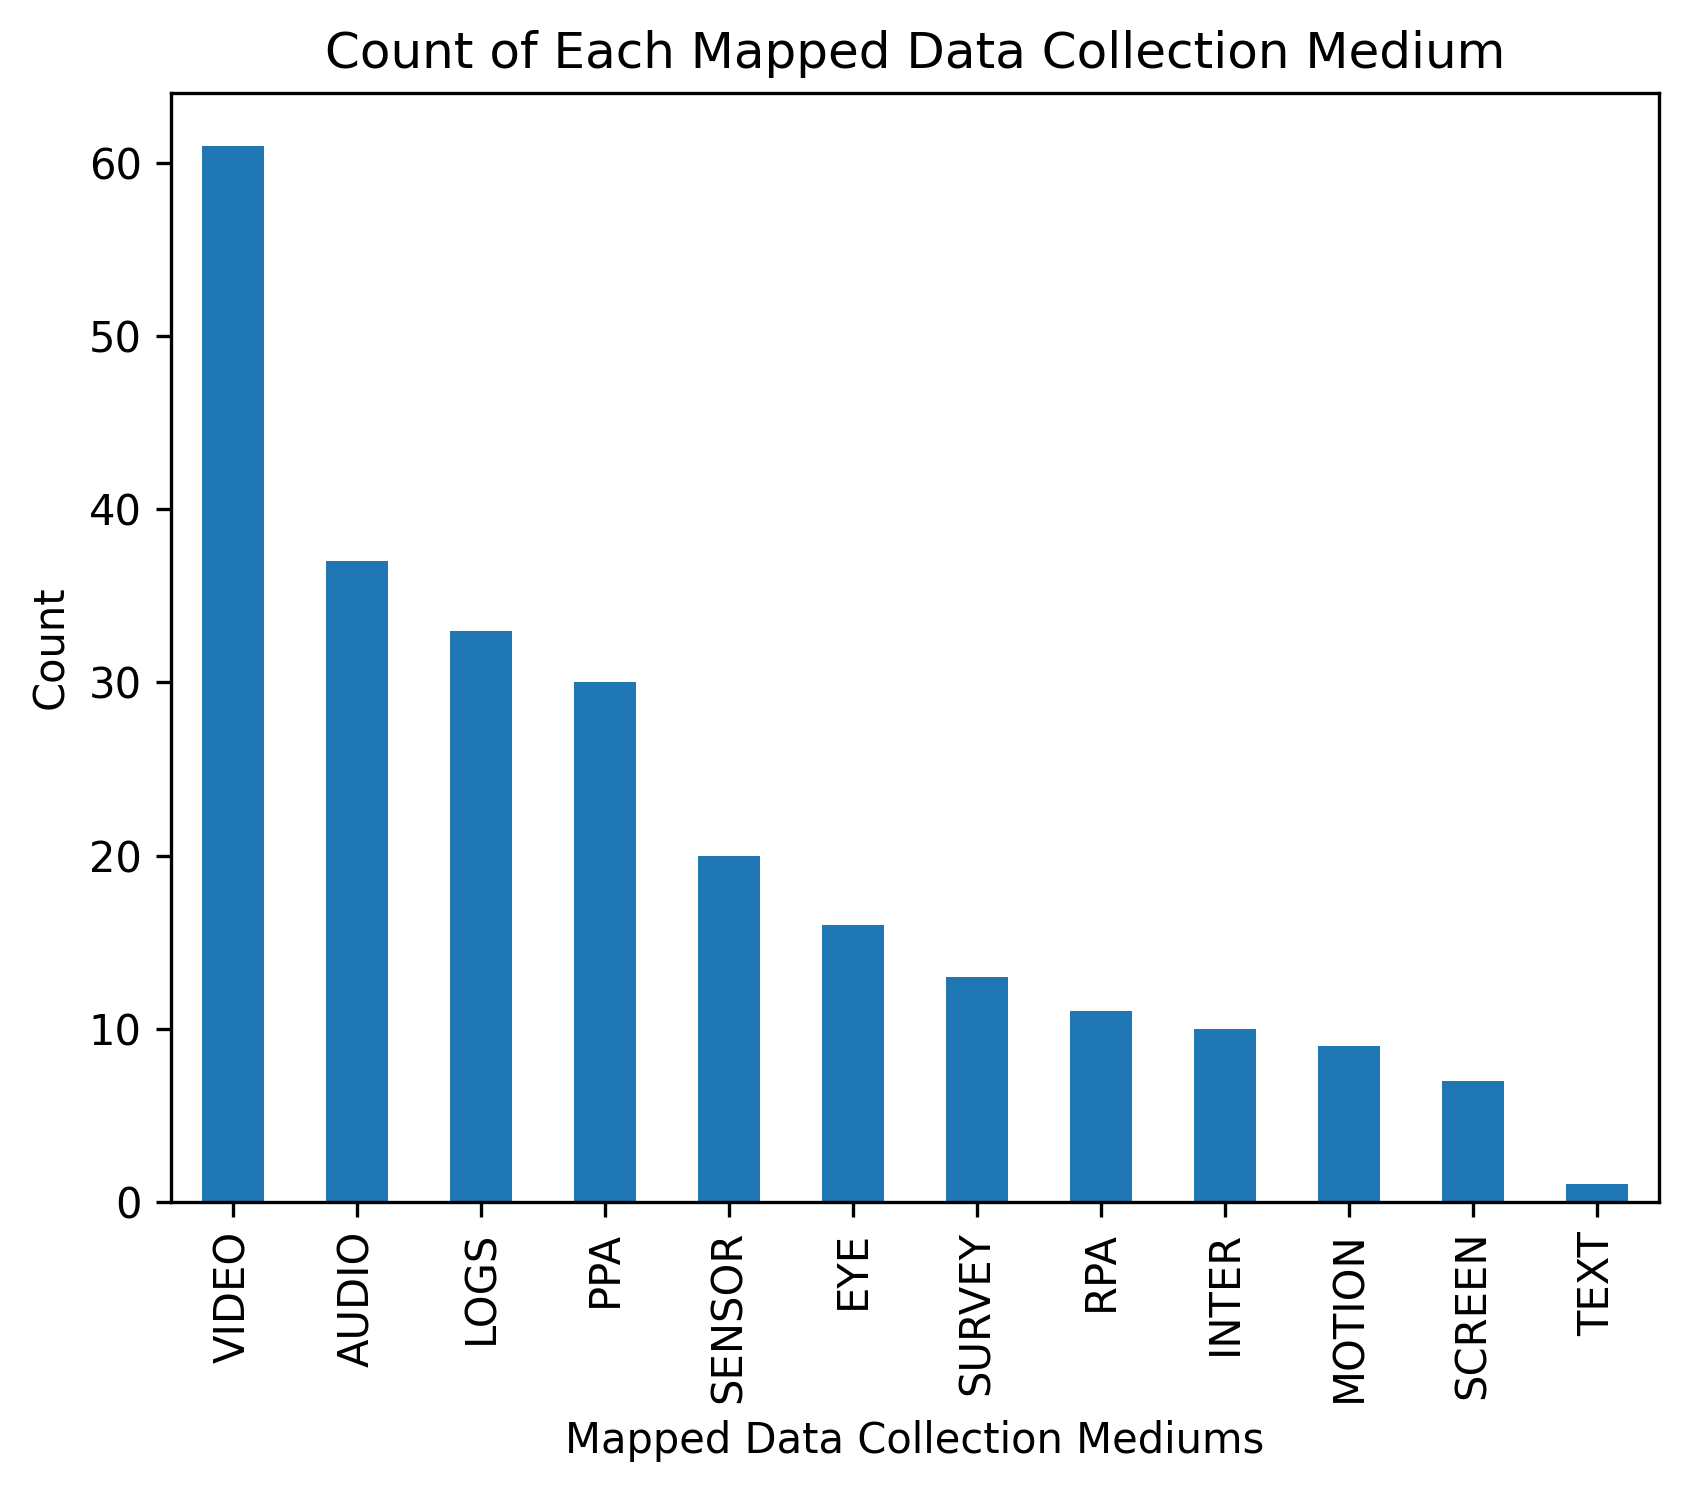
\includegraphics[width=0.5\textwidth]{img/statistical_imgs/data_collection_mediums.png}
  \end{center}
  \caption{Data collection mediums distribution.}
  \label{fig:data_collection_mediums}
\end{wrapfigure}

As depicted in Figure \ref{fig:data_collection_mediums}, the current state-of-the-art in data collection mediums reflects a diverse array of technologies and methodologies, with video (VIDEO) leading at a count of 61, followed by audio (AUDIO) at 37. These two mediums indicate a preference for rich multimedia data that can capture the complexity of learning and interaction in the environments. Logs and participant produced artifacts (PPA) are also popular, with counts of 33 and 30, respectively, suggesting a strong inclination toward capturing learner behaviors and outputs directly from both the environments and the participants themselves.

Despite these advancements, the field faces challenges in integrating data from disparate sources and ensuring data quality and privacy. For instance, sensor data (SENSOR), which has a count of 20, presents challenges in standardization and interpretation. Although less prevalent, eye-tracking (EYE) and motion capture (MOTION) data raise concerns about intrusiveness and the need for sophisticated analysis techniques.

There are notable gaps in text-based data (TEXT), with only one paper \cite{666050348}, indicating a potential underutilization of text-based linguistic analysis in educational research. Additionally, integrating multimodal data streams to provide holistic insights remains an area ripe for exploration. The relatively lower usage of surveys (SURVEY) and interviews (INTER) suggests a research gap in understanding subjective experiences and qualitative dimensions of learning.
% SOTA
% Challenges
% Research gaps

% Descriptive statistics for:
%   Data Collection Mediums

\subsection{Multimodal Data}
We present the breakdown of the different modalities used in our corpus in Figure \ref{fig:modalities}.

\begin{figure}[htbp]
    \centering    
    \begin{subfigure}[b]{0.45\textwidth}
        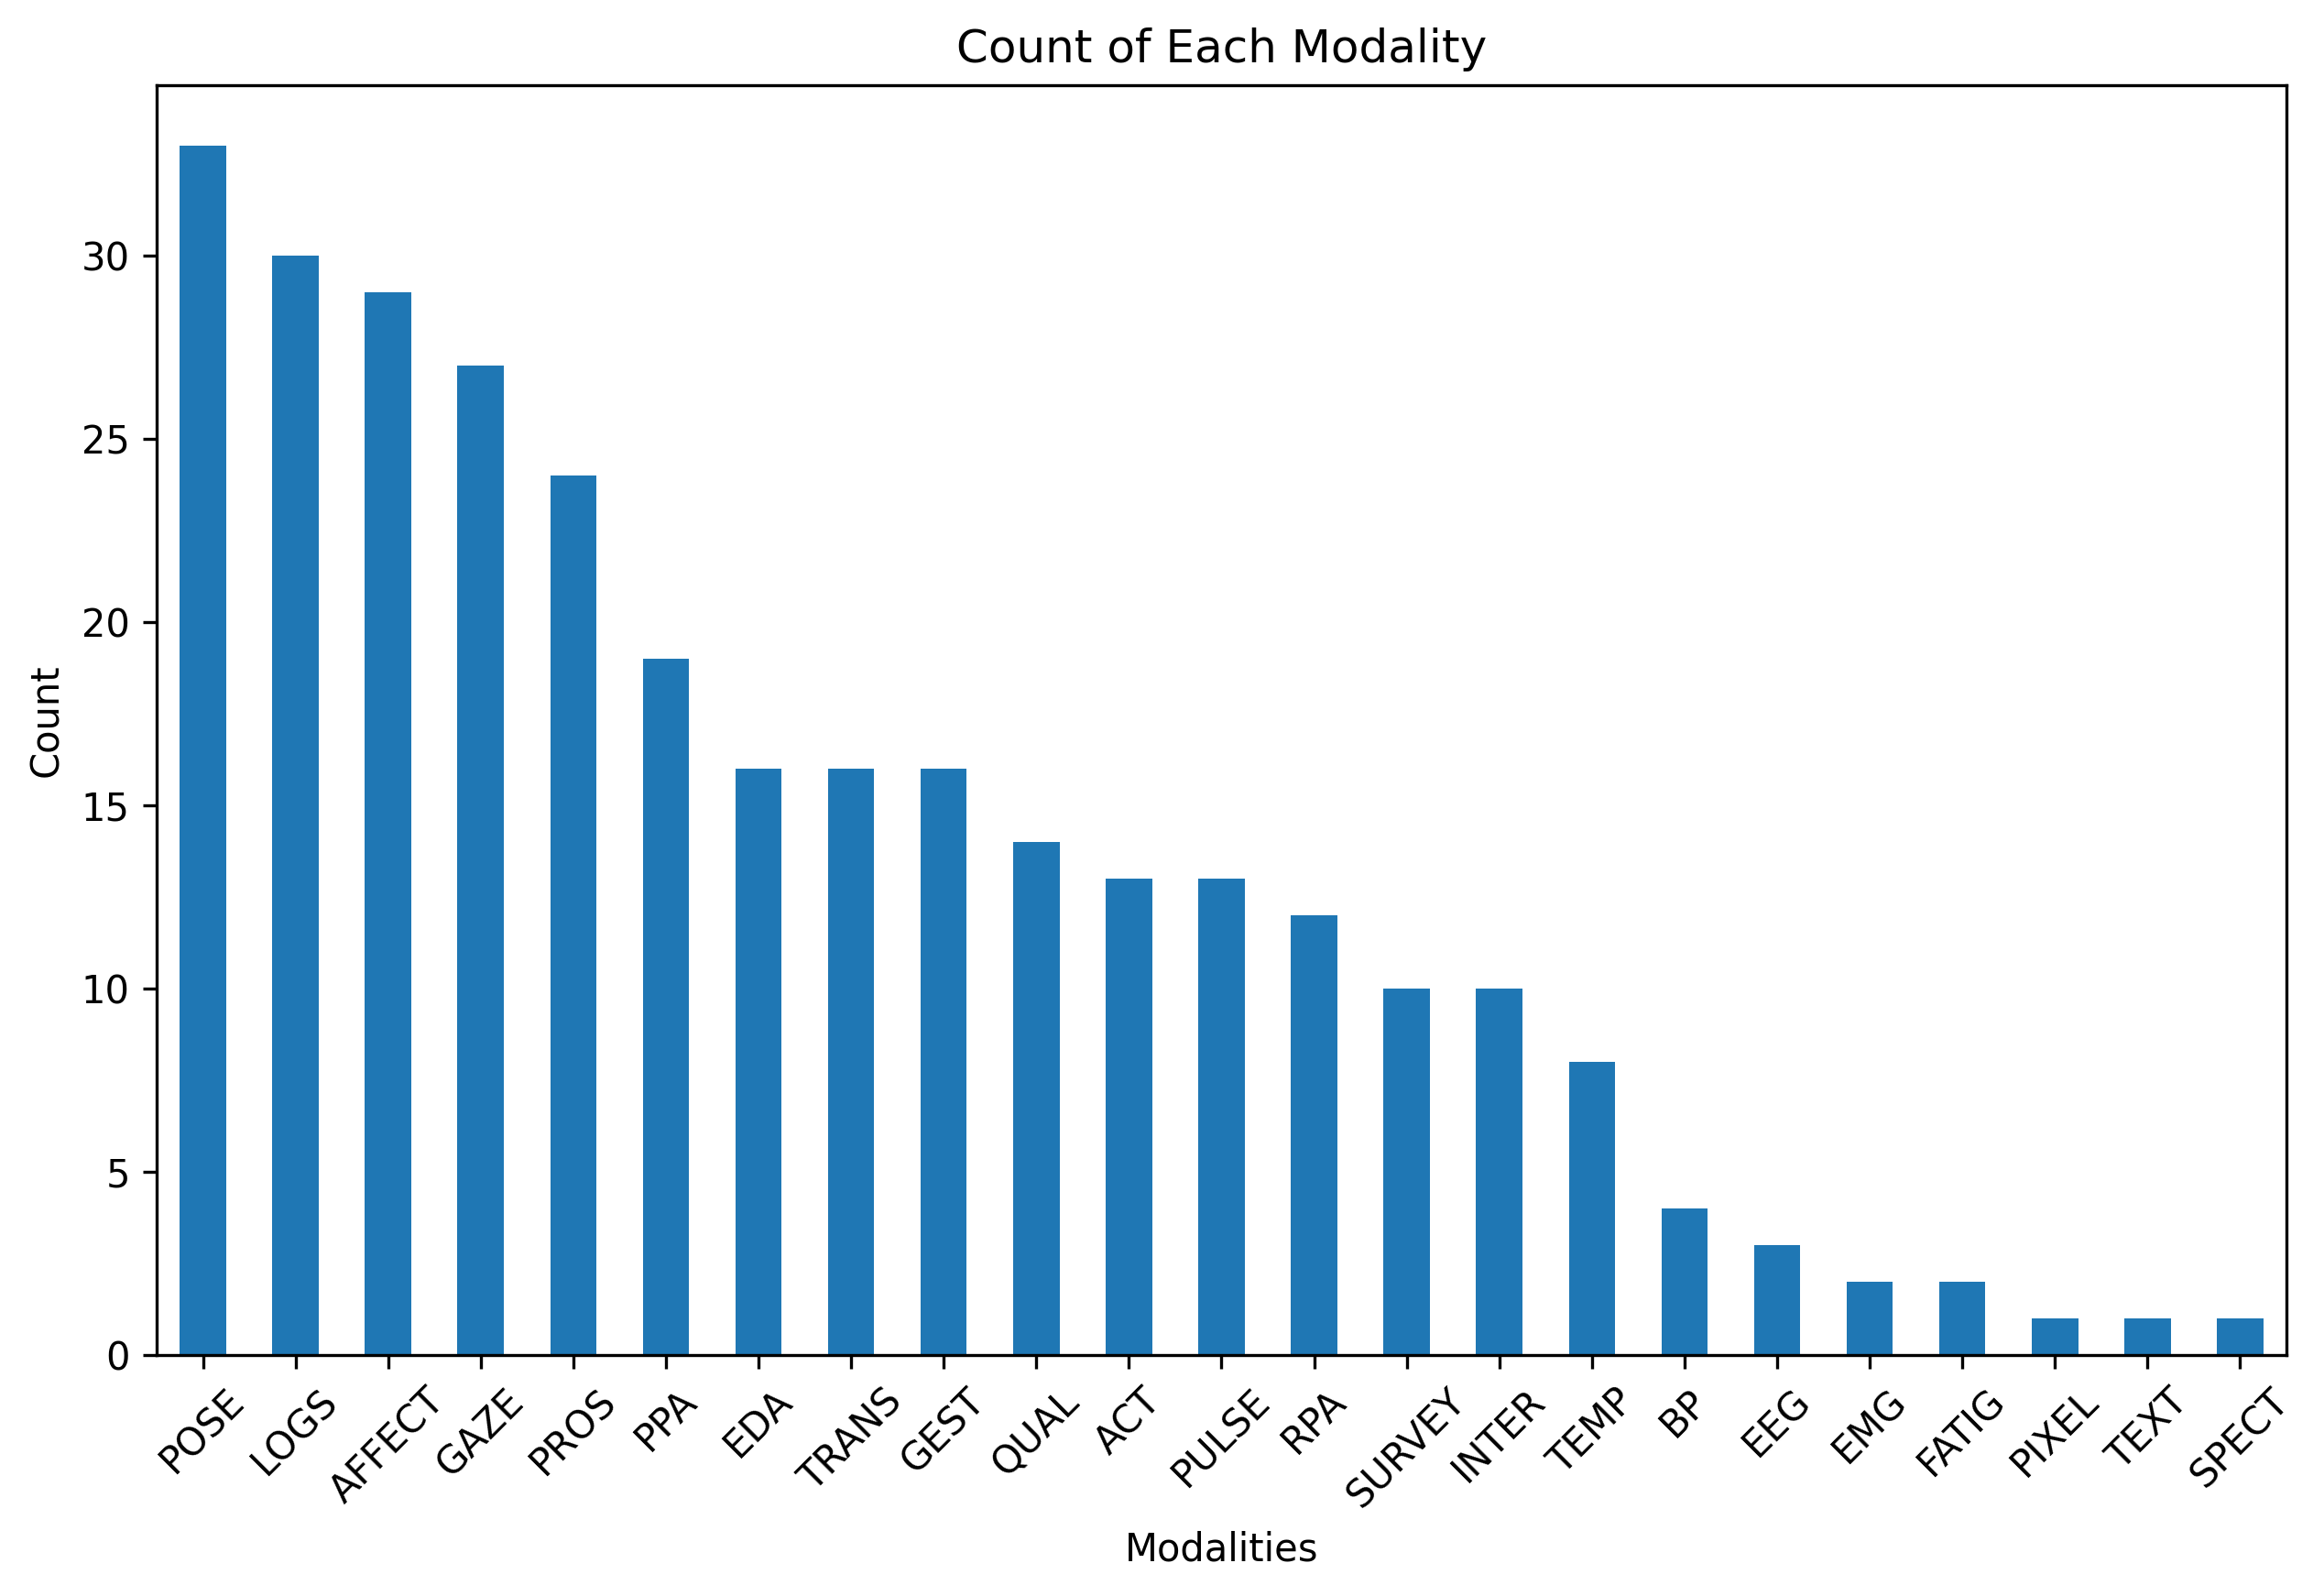
\includegraphics[width=\textwidth]{img/statistical_imgs/modalities.png}
        \caption{Frequency counts for the number of papers in our corpus containing each modality.}
        \label{fig:modalities_freq}
    \end{subfigure}
    \hfill
    \begin{subfigure}[b]{0.45\textwidth}
        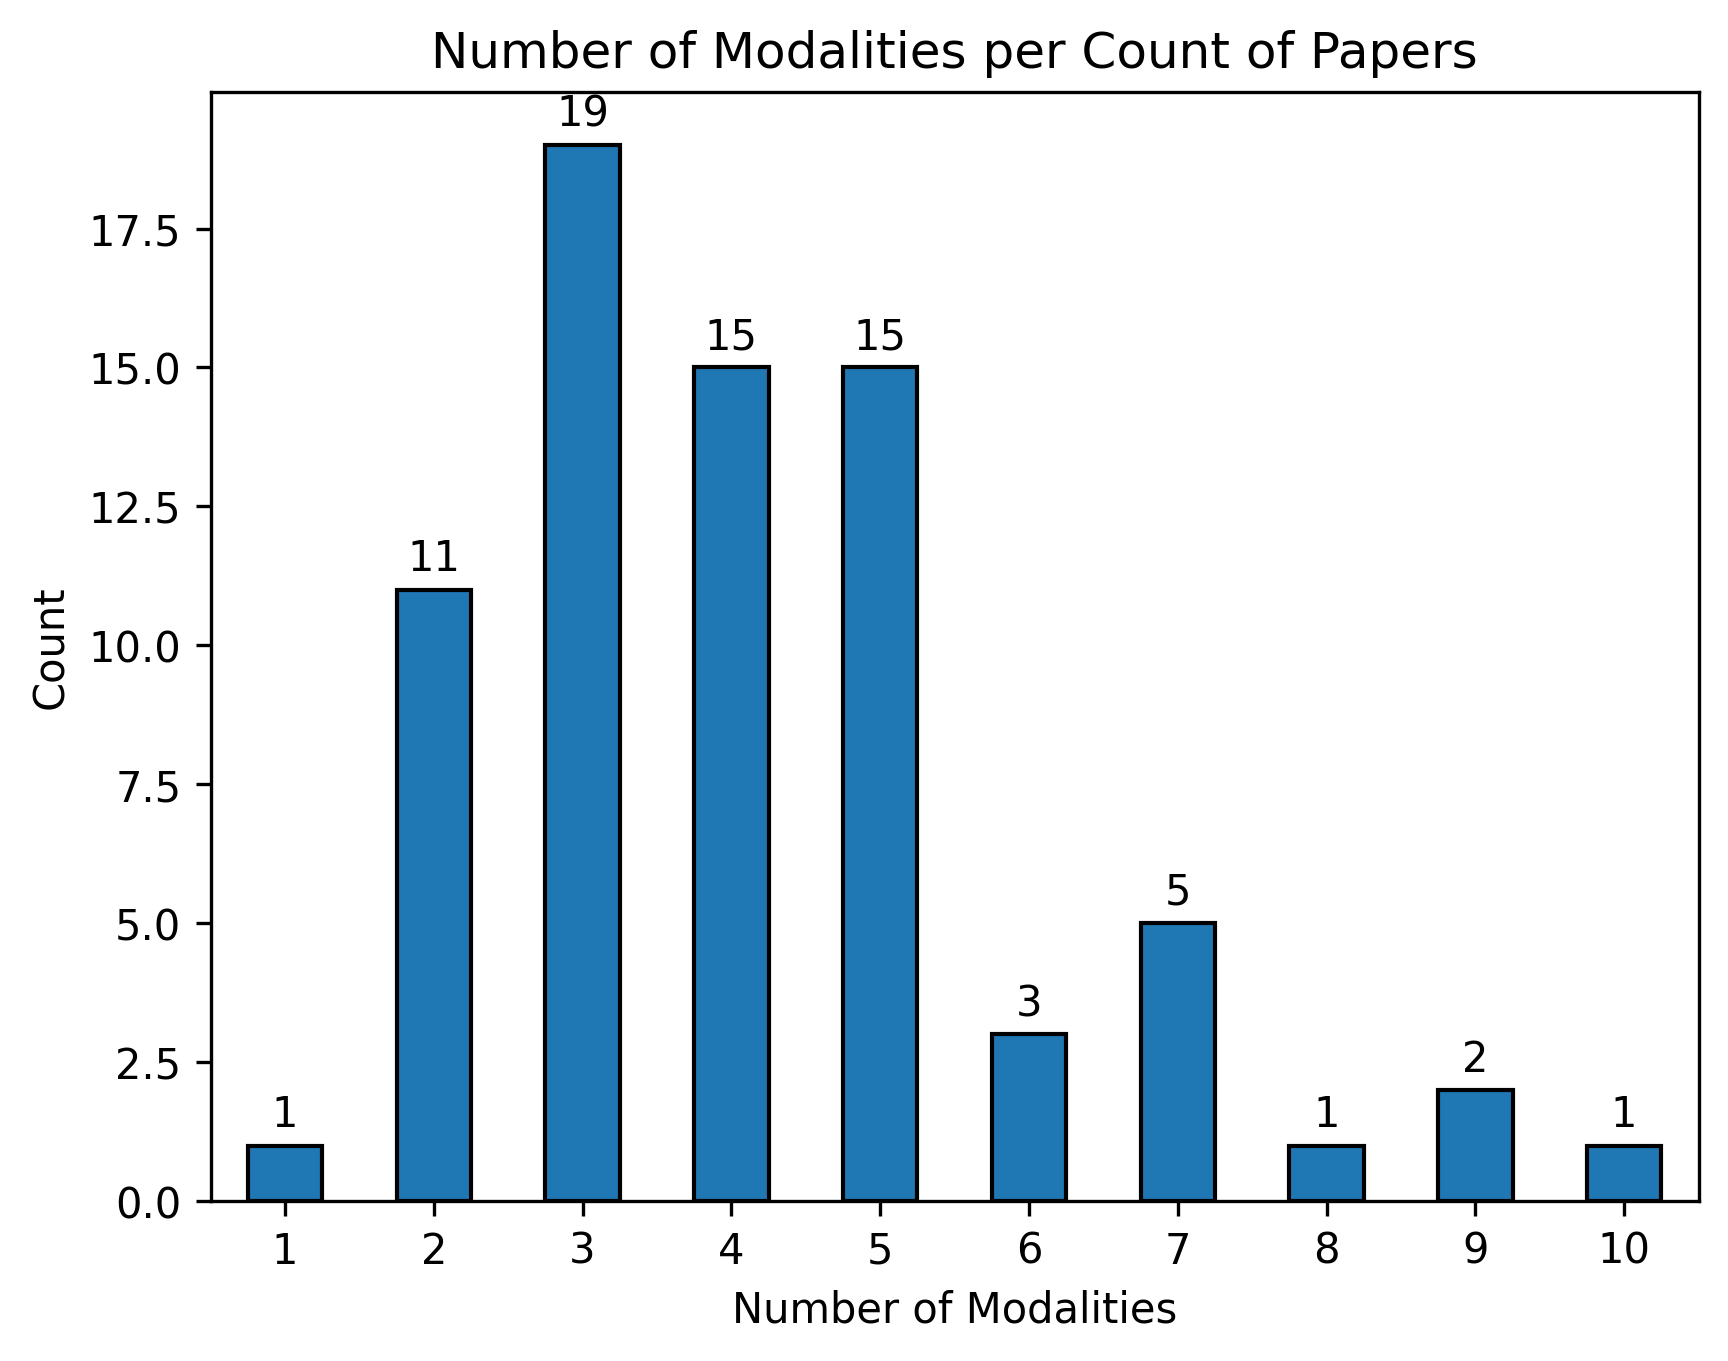
\includegraphics[width=\textwidth]{img/statistical_imgs/number of modalities per count of papers.png}
        \caption{The number of modalities used per paper (i.e., how many papers (y-axis) used $n$ modalities (x-axis)).}
        \label{fig:modalities_nums}
    \end{subfigure}
    \caption{A breakdown of the individual modalities used in our corpus both in terms of frequency count (left) and the number of modalities used per paper (right).}
    \label{fig:modalities}
\end{figure}

``Pose" is the most prevalent modality, appearing in some form in the multimodal pipelines of roughly 45\% of the papers in our corpus. Pose refers to both physical body pose and geospacial location. The logs, affect, gaze, and prosodic speech modalities are also common. At least one of the top 5 modalities appears in all but 8 papers in our corpus. The remaining modalities appear less frequently, with raw text, raw pixel value, and audio spectogram only appearing in one paper each. The vast majority of papers (60/73) use 2-5 modalities in their multimodal analyses. One paper used only 1 modality\footnote{By our definition of ``multimodal" in Section \ref{sec:framework}, we consider a paper to be multimodal if multiple modalities are used during analysis \textit{or} multiple data collection mediums are used. One paper \cite{3809293172} collected both video and audio data, from which the authors derived a single modality: researcher produced artifacts (RPA). For this reason, there is one paper in our corpus that uses only one modality in its analysis pipeline, which we still consider to be multimodal by our definition.}, and one paper used 10 modalities. We hypothesize that researchers typically choose 2-5 modalities due to that range offering a compromise between overhead and informativeness, as several papers alluded to diminishing returns as more modalities and features were added to the pipeline. In these instances, researchers often first collected the data across several modalities but then reduced their feature space via dimensionality reduction techniques like principal component analysis (PCA). 

Diving deeper into the multimodal data, we identified five subdomains based on the modalities that best characterize the types of data that currently drive the multimodal methods being applied to learning and training environments: natural language, vision, sensors, human-centered, and logs. The following subsections present our findings with respect to each subdomain. For each subdomain, we identify the individual modalities it comprises and discuss our findings with respect to its prevalence in the corpus, current SOTA, challenges faced, research gaps, and results achieved.

\subsubsection{Natural Language}

% Descriptive statistics
% Modalities in natural language subdomain
Of the 73 papers in the corpus, 35 of them collected and analyzed some form of natural language data. The natural language subdomain comprises the following modalities: prosodic speech, transcribed speech, raw text, audio spectogram, and affect (when derived from text or audio). Prosodic speech (present in 24 papers) and transcribed speech (present in 16 papers) were the most prevalent natural language modalities, at least one of which appeared in all but 3 of the 35 natural language papers. 8 papers used a combination of prosodic speech and transcribed speech, while 24 papers used one or the other. Only one paper used raw text, and only one used an audio spectogram. 2 papers used audio-based affect. The prevalent natural language features included text-based features taken from transcribed speech (such as n-grams and token counts) and audio-based features taken from prosodic speech (such as volume, pause counts, and pitch variation). 

The majority of natural language papers performed analysis qualitatively or via statistical methods (e.g., correlating features to each other, correlating individual features to outcomes such as learning gains, and performing significance testing). The focus on statistical analysis methods also caused papers using natural language to favor a higher percentage of model-free analysis approaches ($\approx$41\%) compared to the corpus as a whole ($\approx$32\%). Qualitative analysis was particularly prevalent in papers using natural language relative to the corpus as a whole. Of the 73 papers in the full corpus, 9 of them perform qualitative analysis as their lone analysis method, and 7 of those 9 incorporate some form of natural language. 40\% (14/35) of papers using natural language performed classification. This is in contrast to the $\approx$53\% (39/73) of papers that performed classification across the entire corpus, where classification was the most prevalent analysis method overall (discussed in Section \ref{subsec:findings_analysis}). Other analysis methods such as regression, clustering, pattern extraction, and network analysis were used, but only in a handful of instances.

60\% (21/35) of papers using natural language incorporated some form of data fusion, relative to the $\approx$74\% (54/73) of papers in the entire corpus that employed data fusion. Only 19 papers in the corpus did not use (or disclose using) any form of data fusion in their multimodal pipeline, 14 of which were papers using natural language. Among the papers using natural language with data fusion, mid fusion was the most prevalent, appearing in 12/21 papers. Early, late, and hybrid fusion were also used, but only occasionally. In addition to data fusion, another major difference between the full corpus and the papers using natural language is the participant structure. Overall, the ratio of multi-person environments to individual environments in the full corpus is $\approx$2:3 (31:45); however, with the papers that use natural language, that ratio increases to $\approx$5:3 (23:14)\footnote{Some papers analyzed data from both individual and multi-person environments.}. This is largely due to many natural language papers focusing on collaborative learning and training (e.g., collaborative discourse), which necessitates multi-person environments. This is further evidenced by virtual-only environments making up a smaller percentage of natural language papers ($\approx$37\%, 13/35) relative to $\approx$42\% (31/74) in the full corpus, which suggests the majority of collaborative multimodal learning and training research is conducted with a physical component. 

There were no significant differences between the natural language subdomain and the full corpus in terms of didactic nature and level of instruction. STEM was the most prevalent environment subject in environments leveraging natural language modalities, followed by humanities in a distant second, which was also the same for the corpus as a whole. Psychomotor skills was noticeably absent from the natural language papers; however, this is not surprising given all five psychomotor skills papers in the corpus only address individual participant structures and, therefore, do not involve collaboration.

% SOTA
Regarding the current SOTA, traditional machine learning (ML) methods were the most prevalent quantitative approaches in the natural language corpus outside of statistical analyses. In particular, support vector machines (SVMs) \cite{3754172825,85990093,1637690235} and logistic regression models \cite{957160695,3796180663,1576545447} were very often used with natural language features as input. Other approaches like random forest \cite{2273914836}, linear regression \cite{1118315889}, and naive Bayes \cite{1637690235} were also used, typically, to classify (or regress) outcomes such as learning or training gains. Other approaches, such as clustering \cite{2273914836}, extracting behavioral profiles \cite{2273914836}, social network analysis \cite{2345021698}, and Markov chains \cite{3135645357}, were used sparingly. Qualitative analysis typically involved presenting descriptive statistics, case studies, and researchers' observations; and performing thematic analyses \cite{braun2012thematic}, using the constant comparative method \cite{glaser1965constant} to analyze field notes and surveys, and conducting other forms of qualitative coding \cite{2497456347,1847468084,1296637108}.

% Results
Incorporating natural language features in multimodal analysis pipelines consistently yielded positive results. Researchers were able to both correlate natural language features to outcomes (e.g., learning and training gains, confidence, behaviors, strategies, collaboration quality, etc.) and use natural language features to predict these same outcomes. This was particularly true for papers that focused on collaborative learning and training, as the affordances of collaborative (i.e., multi-person) environments offered an additional dimension (discourse) from which to extract features. A large amount of natural language works focused on collaboration \cite{1118315889,3095923626,1637690235}, which was often investigated as both an independent and dependent variable. In collaborative environments, natural language features often showed themselves to be the most informative relative to features derived from other modalities:

\begin{quote}
    The verbal data allowed authors to identify linguistic features in students' collaborative dialogue that were highly predictive of math performance on pretest and posttest assessments, above and beyond any nonlinguistic variables. \cite{3796180663}
\end{quote}

\noindent Additionally, natural language features were generally (although not always \cite{1770989706}) the most predictive when combined with features derived from other modalities. This reinforces findings from previous works, where multi-modal data harnessed more predictive power than any individual modality \cite{sharma_multimodal_2020}. While the combinatorics do become an issue when selecting the most effective feature combinations, researchers reported that including natural language features in the multimodal pipeline often led to improved predictive performance:

\begin{quote}
    Assessing the relation of dual gaze, tutor log, audio and dialog data to students' learning gains, we find that a combination of modalities, especially those at a smaller time scale, such as gaze and audio, provides a more accurate prediction of learning gains than models with a single modality. \cite{3051560548}
\end{quote}

\noindent Overall, the results reported in the natural language papers in our corpus paint a clear picture that natural language features are: 1) often identified as having high correlations with various outcomes, and 2) more powerful in their predictive capabilities when combined with features derived from other modalities. 

However, despite the promising results achieved with natural language, there exist several challenges. Complex natural language tasks characterizing persuasive speech and understanding natural oral arguments in debate are nontrivial and often difficult with contemporary NLP methods \cite{85990093}. Issues with hardware and NLP method limitations also result in data loss or obfuscation before researchers even have an opportunity to conduct analysis. In particular, several natural language papers explicitly mentioned automatic speech recognition (ASR) as being an enormous bottleneck in multimodal pipelines using transcribed speech \cite{1118315889,666050348,32184286}. Learning and training environments are often noisy, consisting of several groups of students or trainees trying to complete tasks simultaneously. This creates environments that are quite noisy (even chaotic) at times, which prevents ASR models from producing accurate transcriptions and performing diarization. This is particularly an issue for environments with children (i.e., K-12 settings) \cite{32184286}. These issues are amplified for non-English speakers and individuals who speak a language other than English at home \cite{666050348}.

Another major challenge lies in the data, an issue which several natural language papers raised \cite{957160695,3783339081,3796180663}. Education- and training-focused datasets are often small, imbalanced, and rife with slang and domain-specific jargon that language models are unlikely to have encountered regularly during training \cite{cochran2022improving,cochran2023improving,cochran2023bimproving}. These types of issues can make it difficult to effectively fine-tune (or pretrain) language models \cite{cohn2020bert} and other deep and machine learning approaches. These previous findings were backed up by several natural language papers in our corpus \cite{957160695,3796643912,3448122334}. Other data issues include the complexity and time-cost. Many software packages like NLTK \cite{nltk}, openSMILTE \cite{eyben2010opensmile}, and TAACO \cite{crossley2016tool,crossley2019tool} allow for programmatically extracting audio- and text-based features; however, doing so often leads to large, opaque feature sets. One paper extracted 6,405 audio features \cite{3135645357}, for example. However, when done manually, preprocessing and feature engineering can be quite expensive in terms of time and may limit the amount of data that researchers are willing to collect and analyze \cite{32184286}: 

\begin{quote}
     To fully understand the events that unfold even in this small segment of a student's educational experience, a researcher may need to watch screen video data, listen to the audio dialogue several times, and enter behavioural codes into a separate document. Having to do this for every problem and concept students experience over the course of even one class period of learning technology use would be vastly taxing on human time and effort. \cite{3796180663}
\end{quote}

The temporality innate to natural language also creates issues, as adding a time dimension to data can make tasks more complex. One can mitigate this by using atemporal natural language approaches like TF-IDF; however, ignoring the time component of natural language will inherently exclude relevant context. Segmenting temporal data manually is tedious and time-consuming. A standard approach to doing so programmatically is by using a \textit{sliding window} approach, but these segments often lack meaning, as they are separated based on time and not environmental context. Recent works have suggested segmenting based on environment logs \cite{snyder2023using,snyder2023analyzing}; however, much of the segmentation performed in the natural language papers in our corpus was done so manually, which is costly:

\begin{quote}
    ...we also faced difficulties segmenting the audio files in order to obtain the students-only utterances in the interview automatically. Thus, we decided to split the audio manually, which was time consuming and, therefore, led to a lower number of students considered in the applied example. \cite{32184286}
\end{quote}

% Research gaps
In addition to the challenges incorporating natural language in multimodal learning and training analysis, we also identified several research gaps. Only one paper in the entire corpus used raw text as input \cite{666050348}, which was surprising given the prevalence of text-based transformer models like BERT \cite{devlin2018bert} and GPT \cite{radford2019language,brown2020language}. Given the performance capabilities (and ubiquity) of large language models (LLMs) and chatbots like ChatGPT\footnote{\href{https://openai.com/blog/chatgpt}{https://openai.com/blog/chatgpt}}, we imagine that text-based features could be an informative addition to multimodal learning and training pipelines, as the quality of raw text does not rely upon speech transcription software. One potential avenue for this is via multimodal conversational agents, which were also lacking in our corpus. While several works addressed multimodal agents or tutors \cite{3093310941,3783339081,1576545447}, these entities typically acted as evaluators, providing summative performance metrics or canned responses (i.e., one-way recommendations). There were no works addressing multimodal \textit{conversational} agents that, for example, act as peers, mentors, or collaborators, while engaging in conversation with students or trainees.

Additionally, only 8 natural language papers incorporated both transcribed speech and prosodic speech in their analysis. Because prosodic speech is devoid of semantic meaning, and transcribed speech lacks important prosodic information like volume and intonation, combining the two modalities provides a more holistic representation of the natural language subdomain. One core NLP research area that would greatly improve researchers' ability to leverage these modalities simultaneously is \textit{textless NLP} \cite{lakhotia2021generative}, which refers to audio-based language models that consider both prosodies and semantic meaning.

The majority of natural language papers primarily relying on qualitative or statistical analyses was also interesting, as there was a noticeable lack of deep learning approaches. While some papers incorporated recurrent neural networks (usually via LSTM models \cite{hochreiter1997long}), these were a relative rarity. Very few used transformer \cite{vaswani2017attention} models like BERT, which was surprising given their prevalence in NLP during the latter half of the time period we targeted during our literature search (2017-2022). Traditional NLP methods such as TF-IDF and Word2Vec \cite{mikolov2013efficient} were typically only used as baselines to demonstrate the relative performance of another proposed approach. All of this indicates that, at the time of this writing (2023), the multimodal methods using natural language to inform learning and training environments lag behind the current SOTA in NLP, which is largely defined by transformer-based deep and reinforcement learning approaches \cite{touvron2023llama}.

As mentioned earlier, a large reason for this lies in the data. Education and training data is often collected in small quantities \cite{snyder2023using,snyder2023analyzing} that are insufficient for training deep neural networks and statistical machine learning algorithms \cite{957160695}. Additionally, data availability is an issue due to privacy concerns, as much of the data collected in classrooms and other learning and training environments is non-public. While the safety and privacy of study participants is paramount (especially when the study participants are children), the lack of massively-open multimodal datasets collected from learning and training environments makes adopting SOTA NLP approaches exceedingly difficult \cite{3796643912}. Another, arguably more pragmatic, research direction is developing models and algorithms that can better inform learning and training environments with limited amounts of data.

\subsubsection{Vision}
Of all of the 5 groups of modalities into which we broke down our analysis, vision-based modalities were far and away the most utilized, with 59 out of the 73 total papers using some form of vision analysis. When we say \textit{vision}, this encompasses any papers which collected data using cameras or eye tracking devices, and analyzed the data using at least one of the following: pose recognition, affect detection, gesture recognition, activity recognition, fatigue estimation, participant gaze, or raw image pixel data. Gaze, affect, and pose appeared most often, present in 27, 25, and 33 of the 59 papers, respectively. Next was gesture at 16 papers, followed by activity recognition in 11 papers. Finally, fatigue estimation and raw pixel data appeared very infrequently, showing up in 2 papers and only 1 paper, respectively.

This distribution of modalities among the vision subset is largely as expected. Pose appeared the most frequently, which is not surprising since there are many off-the-shelf models for pose recognition based on deep learning methods which can be applied quite easily and accurately to learning and training environment data. Furthermore, many researchers use Microsoft Kinect cameras for recording video, which enables pose recognition using the out-of-the-box API, thus allowing this data to be collected quite easily. Gaze was the next most common modality, which is again unsurprising because of the relatively common usage of specialized gaze tracking hardware devices, such as eye tracking glasses, in our corpus. Affect was the third most common modality, which is most likely again due to the availability of off-the-shelf deep learning models for affect recognition. 

Perhaps most significant among this distribution of modalities within the vision subset though is the least used modality: raw pixel data. When we speak about raw pixel data, we mean that the researchers used the raw, unprocessed image data, such as pixel color values, as input to their primary data analysis methods. Instead, most researchers in our corpus fed the raw images into other processing models, such as pose recognition or affect detection as previously discussed, and then used the resulting features as part of their analysis methods. There are two primary conclusions to be drawn from this pattern. First, this serves to underscore the importance of the new mid-fusion category that we have defined in this work. When analyzing video data quantitatively, researchers are hardly ever doing real early-fusion techniques. Instead, they are most commonly relying on pre-trained models to extract mid-level features, and then fusing the mid-level features. Second, this pattern reveals a mismatch between pure computer vision research and this form of applied computer vision research. The trend in many subfields of pure computer vision research is toward the creation of single-stage models which are often trained end-to-end \cite{carranza2021}. This differs from what we have seen in the MMLA literature, where researchers are tending to apply existing models to extract features, and then training a new model with the extracted features as input. This mismatch can likely be attributed to the smaller sample sizes of applied computer vision datasets, such as MMLA datasets \cite{sharma_multimodal_2020}, but nonetheless represents a strong potential area for further exploration in the MMLA literature.

In regard to analysis methods of the vision subset, there was no significant differences between the frequency of analysis methods found in the vision subset and the full corpus, which is not surprising since the vision subset makes up such a large portion of the full corpus. However, we can see a slight inclination toward the use of quantitative analysis techniques in the vision subset, with only 10 papers using either qualitative analysis alone or qualitative analysis combined with statistical techniques. This inclination toward quantitative methods is further reinforced by the slightly higher percentage of model-based methods found in the vision subset ($69.5\%$) when compared to the full corpus ($63\%$). However, despite this leaning toward the use of quantitative methods compared to qualitative methods, the majority of the papers in the total corpus which utilized some form of qualitative analysis (29 papers) also used some form of vision analysis (24 papers). This is relatively unsurprising, given the importance of recorded video data for many forms of qualitative analysis.

Overall, this pattern of analysis methods suggests that there is a lack of mixed-methods analysis occurring. Only 14 out of the 59 papers using vision did a significant combination of qualitative and quantitative analysis. Most commonly, these 14 mixed-methods papers were a combination of classification approaches and qualitative analysis of those classes. In total, this suggests that much of the vision work is methods papers, rather than works aimed at understanding students more holistically or improving learning outcomes. This represents another important area for future work within the vision subdomain: not only should papers be evaluating whether their methods are accurate, but they should also evaluate the effect that such methods could have on a student population. 

% Results achieved
    % Advantages of multi-modal over uni-modal

\subsubsection{Sensors}
% List # of papers falling into this subdomain
% List Modalities
% AFFECT, POSE, EDA, PULSE, ACT, BP, TEMP, EEG, EMG, FATIG, GAZE
% SOTA
% Challenges
% Research gaps

% Results achieved
    % Advantages of multi-modal over uni-modal

Our systematic review identified 20 papers within the realm of sensor-based educational research, covering a spectrum of modalities designed to capture and analyze a wide range of physiological and behavioral data:

\begin{itemize}
    \item AFFECT: 29 papers
    \item POSE: 33 papers
    \item EDA: 16 papers
    \item PULSE: 13 papers
    \item ACT: 13 papers
    \item BP: 4 papers
    \item TEMP: 8 papers
    \item EEG: 3 papers
    \item EMG: 2 papers
    \item FATIG: 2 papers
    \item GAZE: 27 papers
\end{itemize}

Wearable sensors have been pivotal in monitoring learners' emotional and physiological states, predicting behavior and performance, providing real-time feedback, and enabling the integration of multimodal data. Their use extends from classroom environments to specialized training scenarios such as CPR instruction, where they serve not only as tools for assessment but also as mechanisms for adapting educational interventions in real-time.

The integration and interpretation of data from various sensors present substantial challenges, particularly when coupled with the necessity for accuracy and practicality in real-time applications. Ensuring the relevance of sensor data to the learning context and managing the technical complexities of processing multimodal data streams remain significant hurdles.

The advent of advanced predictive modeling, real-time feedback systems, and effective multimodal data fusion represents the state of the art in leveraging wearable sensor data. Yet, there is a pressing need for more granular data analysis to identify subtle patterns and correlations, particularly those not apparent through traditional analysis methods. Contextual and behavioral analytics are required to link physiological responses to specific learning activities in real time.

The field also lacks robust, interactive data visualizations that can intuitively convey complex data sets. Visual correlations with learning events would enable deeper insights, revealing patterns in physiological responses and their triggers. Furthermore, the use of Explainable AI (XAI) methods, particularly attribution-based methods, is scant. These methods could clarify how different sensor data contribute to predictive models, enhancing interpretability in educational research.

Research in sensor-based educational technologies often focuses on immediate or short-term effects; thus, longitudinal studies are needed to assess sustained impacts. Expanding the research to encompass diverse learning contexts and demographic groups will help understand the broader application of these technologies. Moreover, while research often occurs in controlled environments (for example, Manikins), scaling these technologies for widespread use and ensuring their generalizability across diverse educational settings remains a challenge.

Investigations into the user experience and acceptance of wearable technologies in education are also needed, particularly concerning comfort, usability, perceived effectiveness, and most importantly, privacy. These factors are crucial for the successful integration of such technologies into everyday educational practices.

The study conducted by Echeverria et al. \cite{1296637108} stands out in the corpus of literature for its application of accelerometer data to real-world educational settings, marking it as one of the relatively few studies to incorporate such data. Nonetheless, the research is characterized by a narrowed data scope, concentrating solely on accelerometer metrics. Additionally, its reliance on observer-logged data points to the need for a more intricate modeling approach. To achieve a fuller understanding of the learning process through movement and orientation in the setting of CPR simulation, the integration of additional sensory inputs such as gyroscope and magnetometer data might be practical. Such expansion would allow for a multidimensional analysis of physical interactions, potentially unveiling deeper insights into the kinesthetic aspects of learning.

\subsubsection{Human-Centered}
% List # of papers falling into this subdomain
% -TOTAL PAPERS\textbf{ 45} of 73 (QUAL or INTER or SURVEY or RPA or PPA)

% List Modalities
% - QUAL 14, INTER 10, SURVEY 10, RPA 12, \textbf{PPA 19}

% -Out of 45 papers, \textbf{0 have all 5} modalities, \textbf{1 has 4} modalities, \textbf{3 have 3} modalities, \textbf{11 have 2} modalities, \textbf{30 have 1} modality of the 5 (QUAL 6, INTER 3, SURVEY 6, RPA 6, PPA 9)

% -Modalities that appear more frequently together: QUAL + PPA paired in 4 papers, PPA + RPA paired in 4 papers, INTER + QUAL paired in 4 papers

% -Only 1 of 45 papers doesn't have other non-human-centered modalities (it is a paper that does clustering and regression using only RPA)

% - Looking at analysis methods for the 45 papers: \textbf{STATS 22}, CLS 8, \textbf{QUAL 14}, CLUST 5, PATT 7, REG 5, NET 2: using human-centered data for statistical and qualitative analysis predominantly

Out of the 73 papers in your corpus, 45 (approximately 61.6\%) incorporate at least one of the human-centered modalities (QUAL, INTER, SURVEY, RPA, or PPA). This indicates a significant proportion of papers in your corpus that involve human-centered data collection methods. This concentration implies a strong interest in capturing and analyzing data that directly involves human experiences, perspectives, and artifacts, from the perspective of the human who produces the data based on its own interpretations of the tasks taking place during the activity.

Among the human-centered modalities, Participant Produced Artifacts (PPA) has the highest representation with 19 papers, followed by Qualitative Researcher Observations (QUAL) with 14 papers and Researcher Produced Artifacts (RPA) with 12. Interview Notes (INTER) and Survey responses (SURVEY) both have similar representation with 10 papers. 

The prevalence of Participant Artifacts suggests a notable emphasis on utilizing materials produced directly by the study participants. This includes a diverse range of materials, depending on the nature of the study. The high count of Qualitative Researcher Observations indicates a focus on qualitative insights drawn directly from the researcher's observations of participant behavior and the environment.

Among these papers, an overwhelming majority—44 out of 45—incorporate more than one human-centered modality in their analyses, having multiple modalities complement or validate each other, with the exception being a journal article by Closser et al. \cite{3809293172} applied clustering, natural language processing, and general linear modeling to a small dataset comprised of Researcher Produced Artifacts that detailed student behaviors and speech during measurement tasks to identify successful measurement strategies. Amongst the other 44 papers, there is a high variability of combinations of human-centered modalities, with the ones that appear more frequently together being Qualitative Researcher Observations \& Participant Artifacts paired in 4 papers, Participant Artifacts \& Researcher Artifacts paired in 4 papers, and Interview Notes \& Qualitative Researcher Observations paired in 4 papers.

% SOTA
In our analysis of 45 papers employing human-centered modalities notable trends emerged in the choice of analysis methods. A predominant strategy, observed in 22 papers, involves the transformation of human-centered modalities into quantifiable data for statistical analysis. This indicates a statistically significant preference for leveraging these modalities to derive quantifiable insights. Simultaneously, a substantial subset of 14 papers distinctly focuses on qualitative analysis, underscoring a statistically significant emphasis on extracting rich, qualitative insights from human-centered data sources. Further diversifying the analytical landscape, 8 papers engage in classification methodologies, a statistically significant trend in discerning patterns and relationships. Additionally, 7 papers delve into pattern extraction, 5 into clustering, 5 into regression, and 2 into network analysis, showcasing statistically significant variations in the adoption of these diverse analysis paradigms with human-centered data.

Among these 45 papers, a substantial proportion embraces the adoption of multiple analysis methods, highlighting the multi-label nature of this category. Specifically, only 16 papers exclusively employ one type of analysis method, indicating a singular analytical focus. In contrast, 15 papers engage in the integration of two distinct analysis methods, 13 papers exhibit an even more diversified analytical strategy, incorporating three distinct analysis methods. Notably, one paper by Worsley and Blikstein \cite{3095923626} stands out for its comprehensive approach, employing four types of analysis methods to identify correlations between the multimodal data, experimental condition, design quality and learning. The approaches incorporate the use of human-annotated coding of data and automatically annotated data.

% Challenges
While a human-centered approach in multimodal learning analytics brings valuable insights, it also poses several challenges related to subjectivity, scalability, resource intensiveness, and potential limitations in generalizability. Due to the inherent subjectivity of human-centered modalities, the analysis of this data may be susceptible to the influence of the researcher's perspective, possibly introducing bias into the interpretation. Furthermore, these approaches often are resource-intensive, requiring trained researchers for data collection and analysis. Manual collection and human analysis can be time-consuming and may not scale well, especially in large-scale educational settings. Nevertheless, human-centered approaches may offer more transparent and interpretable insights than automated methods.

% Research gaps
While evaluating the use of human-centered modalities, we noticed there exists a noticeable gap in the seamless integration of qualitative and quantitative approaches. While human-centered modalities were frequently employed for either quantitative statistics or qualitative insights, the full potential of these studies could be harnessed by developing methodologies that effectively combine qualitative nuances with quantitative rigor. Secondly, the lack of standardized coding practices for human-centered modalities presents a significant research gap. The absence of common coding conventions across studies hampers replicability and comparability of findings. Establishing standardized coding frameworks proves essential to enhance the reliability and credibility of machine learning analyses, ensuring consistency in the interpretation and utilization of human-centered data. Lastly, a crucial gap lies in the automation of human-coding processes. Most studies relied on manual coding, which is resource-intensive and susceptible to inter-rater variability.

% Results achieved
    % Advantages of multi-modal over uni-modal
Regarding the studies' results, we observed that by integrating multiple modalities, researchers gained a more comprehensive understanding of the learning environment and the learning activities. This human-centered approach offers insights into the participants' experiences, perceptions, and behaviors, often pinpointing subtle nuances that might be missed in a unimodal analysis. QUAL provides rich contextual observations, PPA and RPA offer tangible artifacts, INTER captures in-depth discussions, and SURVEY provides multiple participant perspectives, collectively enriching the analysis. The use of multiple modalities allows for triangulation and cross-verification, where findings from different sources are compared to enhance the validity of the results.
    
\subsubsection{Logs}
% List # of papers falling into this subdomain

% Descriptive in terms of analysis, mediums, modalities, and MF/MB
30 papers (40\%) from the corpus incorporated log data in their analysis -- from now on will be referred to as log-analysis papers. Utilizing logs has a long tradition in both unimodal and multimodal learning analytics. The contents from logs, typically originating from a learning environment/system, provide context for complementary modalities to link them to learning outcomes and performance metrics. We observed that log data is most commonly combined with 3 prevalent data medium groups: multimedia (53\%), qualitative observations (34\%), and sensors (13\%). The high percentage of multimedia mediums points to how an easily interpretable medium, such as video (25\%) or audio (12\%), is a popular approach to supplement logs and address their visibility difficulty weakness. Human-centered artifacts, both from researchers and participants, were less commonly combined with log data compared to the entire corpus distribution. Only 12 log-analysis papers employed sensors in their approach, yet it follows the entire corpus relative trend of low counts of sensor papers. Based on the papers' analysis approach, we split and mapped the corpus into 3 methodology categories: quantitative (QUANT), qualitative (QUAL), and mixed methods (MM). Comparing the log-analysis (QUANT: 40\%, QUAL: 23\%, \& 37\%) and the entire paper corpus (QUANT: 37\%, QUAL: 20\%, MM 43\%), MM decreased by 6\% for log-analysis papers and a minor increase in both QUAL and QUANT of 3\%. In line with quantitative methodologies, the raw output logs of a learning environment are usually not ready for direct analysis, mandating data preprocessing and cleaning. This is congruent with the fusion types data we observed in the log-analysis corpus with zero early fusion and a high concentration of mid and hybrid fusion. Lastly, 23 (72\%) log-analysis papers performed model-based analysis, a 4\% increase compared to the entire corpus, due to a larger emphasis on predicting learning outcomes or variables like engagement.

% Descriptive in terms of setting, participant structure, didactic nature, level of instruction
In terms of the environment and system, only 1 log-analysis paper was performed in a pure physical setting, most of the log-paper corpus generated their logs where the end-user has a direct interface to computer-based systems. 16 (\%53) virtual and 12 (40\%) blended settings log-analysis papers heavily swayed the settings distribution compared to the entire corpus, with the following deltas: virtual (+11\%), blended (+12\%), and physical environments (-25\%). The departure from physical settings indirectly affects the participant structure, causing an increase of individual-focused digital experiences by 11\% amassing 70\% of the entire log-analysis corpus. Digital collaborative environments impose higher engineering and development costs; thereby, virtual and blended studies heavily focus on individual students' trace logs. With more digital-focused settings, the didactic nature of the learning environment also differs from the general corpus. Training settings, more commonly used in training environments, consisted of 5 log-analysis papers, a 4\% decrease compared to the entire corpus. 7 log-analysis papers used informal settings, an increase of 7\% against the general corpus. Lastly, the instructional level of log-analysis papers had no significant trends except for more undergraduate studies (total: 50\%, delta: +11\%). Overall, log-analysis papers are generally computer-based learning environments focused on individualistic instructional or informal activities.

% SOTA (TODO)
For the SOTA in the log-analysis corpus, a variety of methodologies and techniques were employed. The breakdown of the methodologies is the following: 17 (34\%) for classification, 13 (26\%) statistics, 12 (24\%) qualitative, 5 (10\%) regression, 2 (4\%) clustering, and 1 (2\%) pattern recognition. All classification and regression papers used ML algorithms to predict student's achievement, engagement, or emotional state. Classical ML algorithms such as SVM, RF, NB, LR, GB, and MLP \cite{147203129, 483140962, 1019093033%, 1576545447, 1598166515, 1886134458, 2273914836, 2456887548, 2936220551, 3339002981, 3408664396, 3796643912, 4277812050, 1581261659, 3783339081, 4278392816
} were popular to address the small datasets problem and were commonly presented as a bag of classifiers. Only 3 papers superseded traditional approaches to use deep neural networks (DNN) such as CNN \cite{1637690235} and LSTM \cite{2070224207, 3051560548}. Statistical methods were largely used to identify correlations and other descriptive measures between learning variables (e.g. perceived student emotion) to outcome variables (e.g learning gains and achievement). Qualitative approaches consisted of 6 use-cases \cite{666050348, 818492192, 1296637108}, 5 qualitative coding \cite{2273914836, 2936220551, 3856280479}, and 1 interaction analysis \cite{2273914836}. Clustering analysis keenly focused on student \cite{2273914836} and behavior subtyping \cite{818492192} via unsupervised learning algorithms such as KMeans. Pattern recognition only had a single paper \cite{123412197} that used fuzzy set comparative algorithms that embedded qualitative observations to identify combinations/interrelations between variables to explain learning outcomes.

% Challenges
Log data and its analysis are crucial in examining students' digital interactions, yet they encounter various hurdles including issues with time, limited data size, generalizability, and engineering expenses. Temporal aspects introduce notable difficulties in log analysis, such as aligning time frames, handling different sampling rates, and managing time-series data effectively. These temporal complexities make collecting multimodal data a demanding task, often resulting in smaller datasets that limit the scope and scalability of research.

The scarcity of data is exacerbated by challenges in generalizing findings. This is evident in both the log data and the analysis techniques, where models and methods may not seamlessly transfer between diverse learning or training environments. Additionally, the high costs associated with software development and other engineering efforts hinder the integration of innovative and modern features. These features, like real-time collaboration tools in digital spaces (for instance, synchronized cursors, shared documents, and chats), remain limited due to these financial constraints.

% Research gaps
The gaps in log analysis are closely tied to the challenges previously identified, many of which remain unresolved within the multimodal learning and training communities. A substantial portion of research in this field tends to concentrate on overall learning outcomes within an assignment, but often overlooks the nuanced aspects of how student behaviors, emotions, and achievements evolve over time. This oversight represents a significant gap, particularly in the context of piecing together data from various time-scales to construct a more holistic understanding of the student learning process.

Moreover, there is a noticeable rarity in the application of methods and findings from one educational setting to another within the realm of MMLA. This hesitancy is likely attributed to the diverse educational environments and contexts. However, embracing a standardized log format and consistent practices could be a key step in overcoming this barrier. The integration of such standards promises not only more unified research approaches but also the potential for broader applicability of insights and methodologies across different educational scenarios.

Another aspect that underscores this challenge is the low adoption rate of established industry standards like xAPI, LTI, and Learning Management Systems (LMS) within educational technology. This trend reflects a broader issue within the field to align with best practices and norms that have been established in the wider technology and education sectors. Embracing these standards could lead to enhanced interoperability, greater scalability of solutions, and more robust and meaningful analysis of educational data. Ultimately, addressing these gaps and embracing standardization could pave the way for more impactful and transformative educational research and practices.

% Results achieved
    % Advantages of multi-modal over uni-modal
    
\subsection{Data Fusion}


% Descriptive statistics for:
%   Fusion Types

In our analysis of the 73 papers within the corpus, we observed diverse approaches to data fusion in MMLA. The choice between different types of fusion depends on the characteristics of the data, the nature of the learning task, and the desired level of integration. Each fusion strategy has its strengths and limitations, and researchers often select the most suitable approach based on the specific requirements of their multimodal learning analytics study. One noticeable thing in this corpus is that a considerable number of papers don't explicitly explain or justify their fusion choices.

Of the 73 papers, 54 perform early, mid, late, or hybrid fusion. The distribution of fusion types reveals that mid fusion is the most prevalent, employed in 27 papers (36.99\%), showcasing its popularity in integrating information from different modalities during the decision-making stage. Hybrid fusion follows closely, with 19 papers (26.03\%) utilizing a combination of early and late fusion strategies. Early fusion is observed in 3 papers (4.11\%), highlighting instances where feature-level integration is advantageous. Late fusion, occurring after separate models are trained, is employed in 8 papers (10.96\%). Moreover, 20 papers (27.40\%) adopt other types of fusion strategies or no fusion.

A noteworthy aspect of our analysis is the existence of multi-label fusion in the corpus, with 4 papers (5.48\%) employing more than one fusion type. Sümer et al \cite{1315379489} employ both early and late fusion while researching the best performing engagement classifiers using facial videos collected in the classroom. Chango et al. employed mid and late fusion\cite{2936220551} while investigating which data fusion approach and classification algorithms would produce the best results from their data for predicting students’ final performance in their courses and employed hybrid and late fusion\cite{4277812050} to test whether the prediction of students' performance in intelligent tutoring systems could be improved by using attribute selection and classification ensembles. Cornide-Reyes et al. \cite{4019205162} focused on the detection of important relationships and characteristics of the collaborative and non-collaborative groups using network analysis and statistics and employed middle and other (qualitative) fusion. This underscores the complexity and adaptability of data fusion strategies in multimodal learning analytics. 

\subsubsection{Early Fusion}
% SOTA
% Challenges
% Research gaps

In early fusion, the joint feature representation encompasses information from all modalities, allowing the model to learn relationships and patterns directly from the integrated features. This approach is beneficial when the modalities provide complementary information. In our corpus the use of early fusion was only employed in less than 5\% of the papers, highlighting that this fusion type may not always be the most suitable approach since a lot of modalities do not provide the necessary information at the raw data level, making early fusion less advantageous. In the papers that did employ it, the analysis methods included classification, clustering and pattern extraction.

\subsubsection{Mid Fusion}
% SOTA
% Challenges
% Research gaps
    % Discuss the need for mid-fusion relative to early fusion

Mid fusion, or decision-level fusion, involves training separate models on individual modalities and combining their outputs at a later stage, typically during decision-making or inference. It is advantageous when each modality requires unique processing, and combining decisions is more effective than early feature integration. This was shown to be the case while comparing the number of papers that employed mid versus early fusion. Overall, the disparity suggests that mid fusion is currently more favored or deemed more suitable for addressing the challenges and objectives in multimodal learning analytics within the analyzed corpus. 

\subsubsection{Late Fusion}
% SOTA
% Research gaps

In late fusion, the models for each modality operate independently until the final decision or inference stage, where their outputs are aggregated. This approach is suitable when modalities are semantically diverse, and their contributions are better understood when combined at a later stage. In our corpus 8 papers employed late fusion, with 3 of them also employing other types of fusion for comparative purposes\cite{1315379489,2936220551,4277812050}. With the exception of 1 paper that did regression \cite{2836996318}, the majority used fusion for classification purposes.
 
\subsubsection{Hybrid Fusion}


\subsection{Analysis}\label{subsec:findings_analysis}
% EDUARDO
% SOTA
% Challenges
% Research gaps

% MB: 46 (63\%), MF: 16 (22\%), MB&MF: 11 (15\%)
In our collection of papers, we found two main methodologies: model-based and model-free. The choice between these depends on the data at hand and the specific research question. Each methodology represents a different approach and can create a divide among research communities. However, they are best used in union to complement each other's weaknesses and strengths. Model-based methods rely on assumptions about how the system works, while model-free methods demand careful attention to data quality and reliability.

Out of our paper set, 46 papers (63\%) use model-based methods, 16 papers (22\%) employ model-free methods, and 11 papers (15\%) use a combination of both. This distribution, with 78\% of papers favoring model-based analysis, indicates a strong preference in the MMLA community for developing models to explain the learning process. On the other hand, model-free approaches, which make up 33\% of the papers, offer a valuable alternative for exploring learning outcomes in a more exploratory manner.

\subsubsection{Model-Based}
% Obtain profiles for MB and MF corpus

Model-based methodologies apply mathematical frameworks to produce results from given inputs, like in ML models. Common analytical methods include classification (38\%), regression (9\%), statistical analysis (19\%), and clustering (7\%). These methods train models using data samples to predict various factors, such as learning outcomes. When qualitative and pattern recognition techniques utilize model outputs to guide their analysis, they are also categorized as model-based. A notable aspect of model-based approaches is their emphasis on individual experiences (65\%) over collaborative ones (35\%). This trend likely stems from the complexities of mathematically representing the intricate social interactions in group settings. Modeling an individual's cognitive, behavioral, and emotional states is challenging enough; thus, accurately reflecting collaborative dynamics in models is mostly confined to a niche within MMLA and social network analysis.

% Mapped Analysis Methods
% {'cls': 34, 'stats': 17, 'qual': 15, 'reg': 8, 'clust': 7, 'patt': 5, 'net': 2}
% {'cls': 38.64, 'stats': 19.32, 'qual': 17.05, 'reg': 9.09, 'clust': 7.95, 'patt': 5.68, 'net': 2.27}

% Participant Structure
% {'individual': 31, 'multi-person': 17}
% {'individual': 64.58, 'multi-person': 35.42}

\subsubsection{Model-Free}
% Obtain profiles for MB and MF corpus

Model-free methods adopt an exploratory and comprehensive strategy, focusing on the relationships between variables without pre-assuming the link between input and output. Predominantly, these methods involve qualitative (46\%), statistical (38\%), and pattern recognition (13\%) analyses. Qualitative methods are employed in scenarios like use case and interaction analysis, where observations and learning theories guide the understanding of the learning process. Statistical and pattern recognition methods provide descriptions and correlation metrics between learning activity and outcomes metrics. Serving as a counterbalance to the limitations of model-based methods, model-free approaches are widely used in collaborative settings. Here, they are instrumental in dissecting social signals and providing insights into the dynamics of collaboration, including aspects of group health and communication.

% Mapped Analysis Methods
% {'qual': 11, 'stats': 9, 'patt': 3, 'reg': 1}
% {'qual': 45.83, 'stats': 37.5, 'patt': 12.5, 'reg': 4.17}

% Participant Structure
% {'multi-person': 9, 'individual': 7}
% {'multi-person': 56.25, 'individual': 43.75}


\subsection{Feedback}

While the focus of this literature review was on MMLA analysis methods, not on feedback mechanisms, nonetheless they represent an important component of the full MMLA architecture and warrant at least some discussion. In our conceptualization of multimodal learning analytics and multimodal learning and training environments, feedback is bi-directional process that occurs to close and complete the loop of multimodal analysis. We characterize feedback as \textit{direct} or \textit{indirect}. Direct feedback represents feedback that directly involves the learner or other user of the system, which can take two form. First, the MMLA analysis system can provide direct feedback to the learners or trainees. This is the prototypical type of feedback in the context of a learning or training environment, and represents a way of improving some aspect of the users' performance or other goals. There is a massive body of work that defines and analyzes what is means to give good direct user feedback in a learning or training environment, so a full review is beyond the scope of this review. However, the seminal article by Hattie \& Timperley \cite{hattie2007} and the recent literature review by Adarkwah \cite{Adarkwah2021} are good places to start for interested readers. Second, the user can provide feedback to the MMLA system. This can take many forms, but generally involves the user providing some form of feedback about the system as a whole or about the feedback that the system generates for the user. In either case, this feedback from the user about the system represents an important component of a user-centered design approach \cite{abras2004user}.

Indirect feedback, on the other hand, represents feedback that does not directly involve the end user of the system. Most typically, this feedback represents either knowledge about ways to improve the system design or improved research conclusions. Improved system design feedback generally stems from researchers and system designers watching users interact with the system and gaining new understanding of how to improve these interactions, similar to the user-centered design principles mentioned previously. Improved research conclusions occur when the study of learners and trainees in these environments leads to new understandings of the subjects and their populations. This is, of course, a common and desired outcome of much research in the MMLTE field, and can come in many different forms depending on the specifics of the experimental design. For example, in a methods paper designed to measure student engagement using multimodal data, improved research outcomes might mean that the researchers find a new latent variable that is correlated with engagement and can be used to improve the model. Conversely, in a study about student collaboration, improved research outcomes might mean that the researchers found some new insight into how students are collaborating, leading to improved theoretical models. Regardless of the form that it takes, this type of indirect feedback is critically important for any research study.

\section{Discussion} \label{sec:discussion}

Our findings reveal several clear trends in the methods applied to multimodal learning and training environments as a whole:
\begin{itemize}
    \item \textit{Environments}. Learning environments outnumber training environments roughly 7:2, with the majority of focusing on STEM instruction incorporating at least some virtual component (i.e., VRT or BLND environment settings).
    \item \textit{Participants}. Study participants tend to be either university or K-12 students learning or training in multi-person environments slightly more often than individual environments (3:2).
    \item \textit{Data and Modalities}. Video, audio, environment logs, and participant produced artifacts are the most common data collection mediums; while pose, logs, affect, gaze, and prosodic speech are the most popular modalities. The vast majority of works incorporate 2-5 modalities in their multimodal pipelines, suggesting that it is more useful to focus on a few, meaningful modalities rather than several (potentially uninformative) modalities. A large majority of papers performed at least some type of vision analysis (i.e., used features derived from video or gaze). A majority also incorporated human-centered modalities (e.g., participant/researcher produced artifacts, surveys, interviews, etc.), with all but one incorporating more than one human-centered modality.
    \item \textit{Analysis Methods and Approaches}. Classification, statistical analysis, and qualitative analysis were the most common. Classification was typically used for predicting an outcome (dependent) variable like learning or training gains, while statistical methods were often used to select and correlate features (both with each other and with outcome variables). Qualitative analyses typically involved case study observation, qualitative coding, and thematic analyses. Model-based papers outnumbered model-free ones approximately 3:1, suggesting that the community as a whole prefers to develop models to explain the learning and training processes.
    \item \textit{Data Fusion}. Roughly 3/4 of papers performed either early, mid late, or hybrid fusion. Mid fusion was the most prevalent, followed by hybrid fusion. While not always the case, researchers often stated that fused modalities yielded results superior to unimodal or unfused features, so one should consider exploring data fusion while analyzing multimodal learning and training environments. 
    \item  \textit{Publication Mediums}. The \textit{British Journal of Educational Technology} (BJET) and \textit{International Conference on Learning Analytics \& Knowledge} (LAK) were far and away the two most popular publication mediums represented in our corpus. 8 papers were published via BJET, while 7 were published via LAK. No other journal or conference in our corpus was represented by more than three works.
\end{itemize}

The results of our corpus's papers illustrate that multimodal methods are often successful at both predicting learning and training outcomes, as well as identifying the features that are most important in predicting those outcomes \cite{3339002981,1637690235,3783339081}. Vrzakova et al. also point out that even when multimodality does not improve a model's predictive capabilities, patterns in the multimodal data can still be informative. Often, multimodal patterns help contextualize, and add interpretability to, the unimodal primitives by revealing nuances that are unable to be identified by one modality alone \cite{1770989706}. These same patterns can also highlight performance differences among students and trainees:

\begin{quote}
    Our results demonstrate how NLP and ML techniques allow us to use different modalities of the same data, voice and transcript, and different modalities of different data sources, voice data from interviews, answers to a goal orientation questionnaire, and answers to open ended questions about energy, in order to better understand individual differences in students’ performances. \cite{32184286}
\end{quote}

Human-centered approaches offer researchers the opportunity to dive deeper into the learning and training processes to gain a more complete understanding of participants relative to the environment and learning/training activities. The richness innate to human-centered data --- e.g., contextual observations (QUAL), tangible artifacts (PPA/RPA), participant perspectives (INTER/SURVEY), etc. --- allows researchers to gain unique insights into participants' experiences and behaviors by identifying subtleties that more opaque (often quantitative) approaches may miss. 

Our corpus's results also paint a clear picture that multimodal methods are both better-performing and more informative relative to unimodal approaches. This is largely due to the fact different modalities convey markedly different types of information and create complex representations of learners and trainers much richer than is possible by using only a single modality. Often, combining features from completely separate modalities and data collection mediums proved most effective, which Ma et al. \cite{3754172825} demonstrate via several key findings:

\begin{quote}
    The results showed that Linguistic + Audio + Video (F1 Score = 0.65) yielded the best impasse detection performance...\\

    We found that the semantics and speaker information in the linguistic modality, the pitch variation in the audio modality, and the facial muscle movements in the video modality are the most significant unimodal indicators of impasse.\\

    ...all of our multi-modal models outperformed their unimodal models...
\end{quote}

In one paper, Worsley and Blikstein's ``takeaway" is that there are several strategies for performing multimodal learning analytics, and that many approaches offer a ``meaningful glimpse" into complex datasets that may not readily appear using traditional approaches \cite{3095923626}. However, the added complexity endemic to multimodal data and environments also presents several challenges. Liu at al. \cite{3783339081} mention that ``data from different sources are often difficult to integrate." Because the majority of multimodal learning and training data is temporal, data alignment and sampling rate issues often arise. Aligning data streams, collecting data, and labeling data are (often prohibitively) time-consuming processes, and the richness of multimodal data necessitates ``significant human time and effort" to analyze \cite{3796180663}.  

Perhaps the biggest challenge to the field as a whole is a lack of data. The majority of papers in our corpus performed analysis on small groups of learners or trainees, either via case studies or with classroom-sized cohorts. Small datasets such as these make it very difficult to employ many quantitative algorithms, which explains (at least partially) why few works opted for deep learning approaches. Kubsch et al. referred to the limited availability of data as ``one of the major challenges for building robust and reliable multimodal models" \cite{32184286}. These datasets are also often unrepresentative of the population as a whole, which makes it very difficult to develop scalable and generalizable approaches. Multiple researchers discussed these issues as limitations to their work:

\begin{quote}
    ...the design and sample size of the focus group do not allow us to generalize the results. \cite{2609260641}\\
    
    The limited number of pair work EEs does not allow us to make any strong claims in terms of the framework’s reliability. \cite{2155422499}\\
    
    ...the size of the dataset used is relatively small, and the subject pool is not overly diverse, limiting our ability to explore culture or ethics-related factors in the model reliably. \cite{1426267857}\\
    
    ...training a model on a reduced dataset introduces a bias to the model, affecting the validity of the model’s predictions when the data inputs come from a different distribution than the training set. \cite{32184286}
\end{quote}
     
Unfortunately, there is currently a lack of large, open source datasets that are curated to represent multimodal learning and training environments and their participants. This represents a major research gap in the field. Despite several papers mentioning data scarcity as a noteworthy challenge, no papers in our corpus listed compiling large, open source datasets as a research focus, and very few discussed developing generalizable methods that are designed to work with smaller datasets. Currently, the multimodal learning and training SOTA involves formulating methods in a one-off fashion by developing and leveraging approaches that are not necessarily designed to generalize to other datasets, students, age groups, or domains. Researchers in our corpus also heavily relied on derived, observable features (particularly in computer vision, e.g., affect and pose) as model input, which differs from core computer vision approaches and leaves room for exploring end-to-end model training using raw input values (e.g., pixel values) in the future.  

This indicates that the multimodal learning and training SOTA lags behind much of the core AI and ML SOTA, as many contemporary methods and models are often designed to generalize across different types of tasks, datasets, and domains. For example, GPT-4 was tested on several benchmarks, as well as dozens of AP and professional exams. \cite{openai2023gpt4}. In general, most of the SOTA core AI approaches, such as transformer models and reinforcement learning approaches, are currently not being applied to learning and training environments. Much of this is likely due to resource limitations (e.g., monetary or computational cost) or access limitations (i.e., accessing closed, privately-owned models). Additionally, there are privacy concerns with closed models, as private enterprises may opt to preserve researchers' data locally for model training and improvement. 

Another area where our field lags behind core AI is conversational agents. Despite the prevalence of core AI agent-based research, only a few papers in our corpus discussed agents. Those that did discuss agents did so in terms of evaluation and feedback using rules-based methods or other traditional approaches, and did not employ multi-turn, interactive agents (although one paper \cite{3093310941} did mention exploring this in the future). A large reason for this is that our literature search window closed right before ChatGPT's release, and generative AI was not yet ubiquitous when we conducted our search. While we had expected to see more agent-based works leveraging the previous generation of language models (e.g., BERT \cite{devlin2018bert} and GPT-2 \cite{radford2019language}), we hope that the recent proliferation in generative AI engenders a similar rise in multimodal, conversational agents tailored to learning and training environments.

The lack of standardized coding practices and other protocols represents another gap in the literature. Nearly all papers used their own domain- or task-specific coding scheme to label their data, which makes it difficult for researchers to replicate and compare findings. Developing reliable methods for automating human coding procedures is also a major issue. Additionally, the creation of a standardized log format, coupled with a consistent adherence by the research community, would be of great benefit. Even in instances where industry standards are already established, there is a low adoption rate in the multimodal learning and training community. This reflects a broader issue within the community, as researchers are hesitant to align with the previously established norms of the more catholic computer science and learning science fields.  

There is also a relative dearth of training literature compared to learning literature. Training environments, especially physical ones like rehabilitation therapy and athletic training, were not well-represented in our corpus. This is evidenced by the 3:1 INSTR:TRAIN didactic nature ratio and the fact that only 5 papers in the corpus focused on psychomotor skills as the environment subject. Conversely, while sensor data is commonly collected in training environments, it is often not collected in learning environments. Only 20 out of the 73 papers in our corpus used sensor data in their multimodal pipelines, indicating many papers (particularly those dealing with learning environments) are leaving sensor-based features --- like pulse, blood pressure, and body temperature --- largely unexplored. Additionally, the vast majority of papers opted for either quantitative analysis with programmatically-derived features \textit{or} qualitative analysis with human-derived features. Only 20 papers employed both qualitative and quantitative analyses. We envision mixed methods approaches to be a promising research direction going forward as researchers seek to gain more comprehensive understandings of their study participants' learning and training processes. Lastly, environments focusing on professional development were also a rarity (5 papers); and no papers, to our knowledge, conducted longitudinal analyses of students or trainees across multiple tasks, assignments, or grade-levels. 

\subsection{Limitations}
The major limitations of this work involve the use of Google Scholar to conduct the literature search and the use of a citation graph for programmatic corpus reduction. Both are discussed in the following paragraphs.

\subsubsection{Google Scholar.} While Google Scholar is widely used by researchers across both academia and industry, it poses a challenge for reproducibility. Like Google Search, Google Scholar is a non-deterministic, proprietary search algorithm. Factors such as the individual user conducting the search, the user's geolocation, the date the search was conducted, and the user's search history may all affect how Google Scholar collates search results. Google may also perform A/B testing in live environments to determine which version of its algorithm users deem more effective. The algorithm is also (presumably) continually evolving, and users are unable to know exactly which version of the algorithm is used to conduct a particular search. As such, there is little expectation that our initial corpus will be able to be reconstructed \textit{in its exact form} without at least some degree of variability.

The authors are confident the degree of variability from different Google Scholar searches does not prohibit the \textit{overall} reproducibility of the initial corpus. While SerpAPI's web scrape method is proprietary, the creators address several of our concerns in their documentation\footnote{https://serpapi.com/}. The API's search does not use information from any individual user's Google account when conducting the web scrape, as no Google account is attached to the SerpAPI account, API key, or API calls themselves. Instead, calls are made via proxy and random headers, as illustrated in Figure \ref{fig:serpAPI}. When trying to reproduce the API's results via manual search, SerpAPI recommends using the URL in the API's JSON results in ``incognito mode". 

\begin{figure}
    
\includegraphics[width=\textwidth]{img/SERP_API_diagram.drawio.png}
    \caption{Searching Google Scholar via SerpAPI.}
    \label{fig:serpAPI}
\end{figure}

Additionally, we reached out to SerpAPI directly and asked, ``Does SerpAPI attach personal or identifying information when making request?", to which SerpAPI responded, ``No, we don't add any personal information." SerpAPI also stated, ``...others can reproduce your results by using Google Scholar website, if they use the same search criteria...", but we believe this to be an overstatement given Google's lack of transparency with regard to exactly which algorithm is being used in any single search. While we cannot guarantee perfect reproducibility due to the aforementioned issues, we can state with a reasonable degree of confidence that our own individual search biases did not influence the initial search results (outside of the choosing of the search terms) due to how SerpAPI handles API calls to Google Scholar. For reference, this review's literature search was conducted by an author of this paper in Nashville, TN, USA on October 22, 2022.

\subsubsection{Citation Graph Pruning.} 

As discussed in Section \ref{subsec:study_selection}, we initially pruned our corpus using quantitative means via the use of a citation graph. In doing this, it is possible we excluded relevant works from our corpus based on them only having cited or been cited by a minimal number of other works in our corpus. This literature review is a survey of the prominent methods, practices, and approaches researchers are applying to multimodal learning and training environments. As such, the authors agreed that if a work did not utilize a large degree of previous research (i.e. cite several other works in the corpus) or serve as a base from which a large degree of other researchers have built upon (i.e. be cited by several other works in the corpus), then that work was likely outside the scope of our review. Considering our corpus was still largely comprised (over 50\%) of works later deemed to be outside the scope of this review after graph-based pruning, the authors are confident that few papers directly pertaining to multimodal learning and training environments were discarded as a result of graph-based pruning.

\subsubsection{Other Limitations}.
% Paper that was not peer reviewed (possibly) \cite{483140962}
Other, more minor limitations are also worth mentioning. Due to the prevalence of papers being published to open, non-peer-reviewed platforms like arXiv in recent years (particularly in computer science), we did not screen for non-peer-reviewed works during study selection (i.e., we did not adopt a paper's not being peer-reviewed as an exclusion criterion). There is one paper in the corpus that was submitted to a workshop that none of the authors are familiar with. We are, therefore, unsure of whether or not the paper underwent a formal peer-review. However, the workshop includes submission, notification, and camera ready dates, so we are confident that the workshop is at least refereed to some degree. The rest of the papers in our corpus, to the best of our knowledge, all underwent formal peer-review.

Another limitation is that each of our 42 literature search queries included the word ``multimodal" (in some form). It is possible that works performing multimodal analysis on learning and training environments were unintentionally excluded from our search due to the word ``multimodal" not being explicitly present in their manuscripts. Due to the opacity of Google Scholar's algorithm, we cannot be sure how reliant it is on individual keywords. 

Finally, we conducted our literature search in October 2022---one month before the release of ChatGPT\footnote{\href{https://openai.com/blog/chatgpt}{https://openai.com/blog/chatgpt}}. The increasing degree to which ChatGPT (and other LLMs) are beginning to shape research methodologies is difficult to overstate. Recently (summer of 2023), publications applying LLMs to education- and training-based tasks and environments began to emerge. However, due to the timing of our literature search relative to ChatGPT's release, works in our corpus do not include LLMs in their multimodal pipelines. We anticipate that, as the prevalence of LLMs continues to grow, these powerful models will serve as a foundational piece of many multimodal analysis pipelines used to inform learning and training environments.

\subsection{Future Research Directions} 

The results presented in our corpus demonstrate that multimodal methods can be quite powerful when applied to learning and training environments; however, our analysis of the challenges and research gaps alerts us to several research directions in need of further exploration. We discuss several directions we feel would provide the greatest benefit to the field if pursued. 

\textit{Multimodal LLMs}. The recent boom in generative AI and multimodal LLMs creates tremendous opportunities for multimodal learning and training research. SOTA models like GPT-4 \cite{openai2023gpt4} and Gemini \cite{team2023gemini} allow for prompt engineering approaches that obviate the need for traditional model training (i.e., parameter updates) and large datasets \cite{cohn2023chain}. Smaller, open source models can also be trained via parameter-efficient methods to help east the computational overhead endemic to large transformer models \cite{dettmers2023qlora}. We see both prompt engineering and multimodal conversational agents as two promising research directions, in particular.

\textit{Data Scarcity Mitigation}. Data scarcity is perhaps the most significant issue currently plaguing the field and is responsible for multimodal learning and training methods lagging considerably behind many SOTA core AI approaches. Compiling massively open learning and training corpora could go a long way to help mitigate this, as could designing generalizable approaches requiring limited amounts of data.

\textit{Standardization}. Standardized coding conventions and practices are needed for the field as a whole, particularly for human-centered data and modalities. Establishing these standardized frameworks is paramount to improving the reliability and credibility of machine learning methods, as well as the efficiency of interpreting and utilizing human-centered data. This is also important for log data, as embracing a standardized log format could help the field overcome its reliance on setting-specific methods and improve generalizability. Additionally, it is equally important that researchers make an active effort to adhere to the standards and practices already in place. 

\textit{Active Environments}. Environments where study participants are physically active provide an opportunity for researchers to incorporate motion-based modalities into their multimodal pipelines (e.g., via inertial measurement unit, IMU, sensors). This type of research was largely absent from our corpus, and we envision it being particularly useful to researchers interested in physical training and embodied learning \cite{zhou2023embodiedai}.

\textit{Explainability}. Many AI and ML approaches involve black-box algorithms whose outputs lack explainability. This is problematic, as researchers (and teachers, trainers, study participants, etc.) often cannot understand the model's decision-making processes. This can both hinder teachers' and trainers' ability to guide their pupils, and foment distrust in AI algorithms and systems. Prior works have sought to create more explainable systems via data visualization tools that help make participants' learning and training processes more transparent \cite{hutchins2022co,vatral2023comparative,davalos2023chimerapy}. Some works in our corpus did so as well \cite{2609260641,2879332689}, but more research is needed. We also recognize the potential for LLMs to contribute to enhancing explainability. For example, \textit{Chain-of-Thought} prompting \cite{wei2022chain,cohn2023chain} elicits reasoning chains from the LLM alongside the model's responses.

\textit{Longitudinal Analyses}. The vast majority of studies focus on using multimodality to either predict overall learning and training outcomes or identify the features that correlate with those outcomes; however, these types of approaches to not consider how students and trainees evolve over time. Conducting longitudinal studies would provide insight into how study participants' behaviors and abilities develop as they progress in their learning or training. 

\section{Conclusion}
In this paper, we conducted a comprehensive literature review of the research methods currently being applied to multimodal learning and training environments. In doing so, we developed a novel, programmatic approach to literature review corpus reduction, \textit{citation graph pruning}. We presented a taxonomy and framework reflecting the current advances in multimodal learning and training research, and identified and analyzed five subdomains of multimodal data (Natural Language, Vision, Sensors, Human-Centered, and Logs). We presented descriptive statistics, performed a qualitative thematic analysis, and discussed our findings with respect to the current SOTA, results achieved, challenges faced, and research gaps for both the subdomains and the corpus as a whole. Consequently, we identified the need for a new type of data fusion, \textit{mid fusion}, which is characterized by fusing derived, observable features. We concluded by presenting the limitations of our work and offered several promising avenues for further research exploration. As the field of multimodal learning and training analytics continues to expand with the advent of the generative AI era, it is our sincerest hope that this literature review will serve as a springboard for new multimodal learning and training methods and research.

\section*{Conflict of Interest Statement}
The authors have no known conflicts of interest to declare. 

\begin{acks} 
This work is supported in part by the National Science Foundation under awards XXX-XXXXXXX and XXX-XXXXXXX.
\end{acks}

%%
%% The next two lines define the bibliography style to be used, and
%% the bibliography file.
\bibliographystyle{ACM-Reference-Format}
\bibliography{references, zotero_references, uuid_references}

%%
%% If your work has an appendix, this is the place to put it.
% \appendix

\end{document}
\endinput
%%
%% End of file `sample-manuscript.tex'.